\section{Introduction}
The aim of this chapter is to show the characteristics of the new detectors presented for the upgrade of ATLAS detector,
and how they can achieve the requirements for the high luminosity events.
The results of each test to characterize the detector are presented in this chapter.


\subsection{High Luminosity Large Hadron Collider}
The Large Hadron Collider (LHC), run by the European Organization for Nuclear Research (CERN, derived from {\it Conseil
Europ\'een pour la Recherche Nucl\'eaire}) at the Franco-Swiss border near Geneva, a circular accelerator with 27km of acceleration pipes, is the largest scientific instrument ever designed and built for scientific research.
It has been successfully commissioned in March 2010 for proton-proton collision with a \SI{7}{GeV} center-of-mass energy.\\ 
The LHC is pushing the limits of human knowledge, enabling physicists to go beyond the Standard Model (SM): the enigmatic
Higgs boson, the mysterious Dark Matter and the world of super symmetry are just three of the long-awaited mysteries that
the LHC is working to unveil. \par
The announcement given by CERN on 4 July 2012 about the discovery of a new boson at 125-126GeV\cite{atlas,cms}, almost certainly
the long awaited Higgs particle, is the first fundamental discovery, hopefully the first of a series, that the LHC can
deliver.\\ Such discovery was made possible thanks to the general-purpose detectors ATLAS and CMS, both located at 4
interaction points together with the detectors ALICE and LHCb.\par



% -------- LHC Schedule Table ------ 
\begin{table}[h]\footnotesize
\centering
\begin{tabular*}{0.8\textwidth}{rcccc}
\cellcolor{blue} &\cellcolor{blue}\textcolor{white}{Period} &\cellcolor{blue}\textcolor{white}{Energy $\sqrt{s}$} &\cellcolor{blue}\textcolor{white}{Luminosity ${\cal
L}$} &\cellcolor{blue}\textcolor{white}{Integrate ${\cal L}$} \\
\cellcolor{cyan} \textcolor{white}{Run I} 	& 2010-2012 & 7-8 TeV & \SI{6e33}{cm^{-2}s^{-1}} & \SI{25}{fb^{-1}}\\
\cellcolor{cyan} \textcolor{white}{LS1} 		&\cellcolor{lightgray}2013-2014 & \multicolumn{3}{l}{\cellcolor{lightgray}Go to design energy, nominal luminosity,
bunch spacing 25ns}\\
\cellcolor{cyan} \textcolor{white}{Phase 0} & 2015-2018 & 14 TeV & \SI{1e34}{cm^{-2}s^{-1}} & \SIrange{75}{100}{fb^{-1}}\\
\cellcolor{cyan} \textcolor{white}{LS2} 		&\cellcolor{lightgray}2019-2020 & \multicolumn{3}{l}{\cellcolor{lightgray}Upgrade muon spectrometer;NSW,LAr
Calorimeter \& FTK}\\
\cellcolor{cyan} \textcolor{white}{Phase 1} & 2021-2023 & 14 TeV & \SI{2e34}{cm^{-2}s^{-1}} & $\sim$\SI{350}{ fb^{-1}}\\
\cellcolor{cyan} \textcolor{white}{LS3} 		&\cellcolor{lightgray}2024-2025 & \multicolumn{3}{l}{\cellcolor{lightgray}New Inner Tracker and trigger
architecture}\\
\cellcolor{cyan} \textcolor{white}{Phase 2} & 2026-2030 & 14 TeV & \SI{5e34}{cm^{-2}s^{-1}} & $\sim$\SI{3000}{fb^{-1}}\\
\end{tabular*}
\caption{LHC Schedule }\label{lhcschedule}
\end{table}


\subsection{ATLAS Detector}
The ATLAS detector is a general-purpose detector, designed to explore proton-proton collisions at center of mass up
to $\sqrt{s}=$14GeV in the Large Hadron Collider (LHC) at the European Laboratory for Particle Physics (CERN). It is
aiming to understand the foundations of matter and forces, in particular the nature of mass in a broad physics
program. The ATLAS detector was built with the ability to discover the Higgs boson over a wide mass range. It can also
perform searches for the production of heavy particles that would indicate physics beyond the Standard Model, such as
super symmetric particles, as well as searches for other massive objects. \par 
To be able to detect such important and rare events, this machine has multiple and complex detector systems. In the
central part of this cylinder lies the Inner Detector, the first part of ATLAS to see the decay products of the
collisions, and as such, very compact and highly sensitive component. It consists of three different systems of sensors, all immersed
in a magnetic field parallel to the beam axis. The {\bf Inner Detector} measures the direction, momentum, and charge of
electrically-charged particles produced in each proton-proton collision. The next part is the Calorimeter (red and green
on figure ~\ref{fig:ATLAS}), which  measures the energy of a particle when it loses its energy as it passes through the
detector. It is usually designed to stop entirely or ``absorb" most of the particles coming from a collision, forcing them
to deposit all of their energy within the detector. Calorimeters typically consist of layers of ``passive" or
``absorbing" high-dense material -for example, lead-interleaved with layers of an ``active" medium such as solid
lead-glass or liquid argon.\par
\begin{figure}[ht]
		\centering
		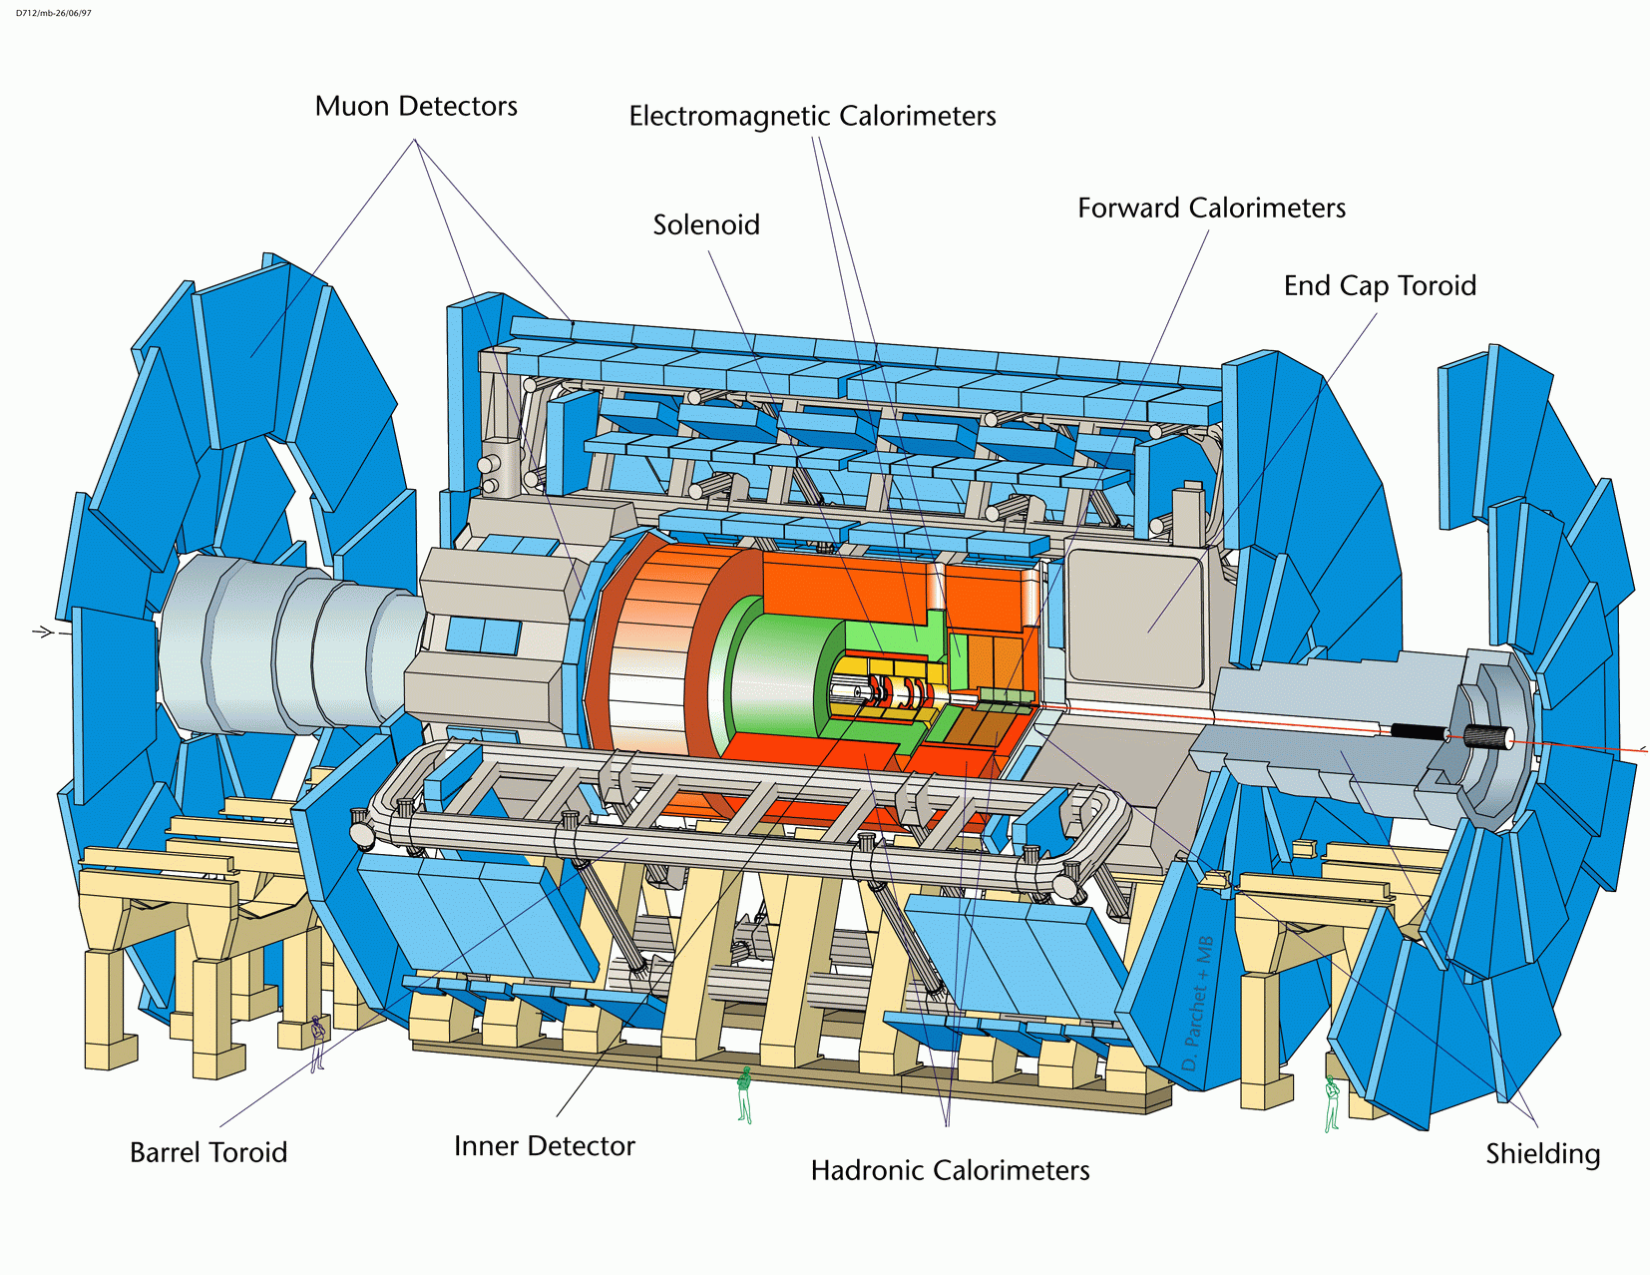
\includegraphics[width=0.7\textwidth]{ATLAS.pdf}
		\caption{ATLAS detector, Muon Spectrometer (in blue)}\label{fig:ATLAS}
\end{figure}
Electromagnetic calorimeters measure the energy of electrons and photons as they interact with matter. Hadronic
calorimeters sample the energy of hadrons (particles that contain quarks, such as protons and neutrons) as they interact
with atomic nuclei. The components of the ATLAS calorimetry system are: the {\bf Liquid Argon (LAr) Calorimeter} and the
{\bf Tile Hadronic Calorimeter}.\par

Calorimeters can stop most known particles except muons and neutrinos. Muons are particles that usually pass through the
Inner Detector and Calorimeter undetected, they can penetrate through large amount of material without any strong
interaction, they have long lifetime, therefore, can be considered as stable particles within detector's volume, offering lepton decay channels for heavy objects as:\par
%$H\rightarrow \mu^+\mu^-$, $W\rightarrow \ell^-\ell^+$

\textcolor{red}{ADD lepto-production from heavy particles}
\par
To detect these particles, the ATLAS detectors use the {\bf Muon Spectrometer}, made up of 4.000 individual muon chambers
(different types of drift
chambers) which are in charge of identify each one of these muons. However, it is only possible to measure its momentum with the help of the {\bf
Magnet System}, made of three sections; the {\bf Central Solenoid Magnet} with 2T
magnetic field bends the
charged particles for momentum measurement near the interaction points, helping the Inner Tracker system, the {\bf
Barrel Toroid} bends the particles with low transversal momentum, and the {\bf Endcap Toroid} with 4T magnetic field takes part in the
high transverse momentum.\par
% -------------------------------------- Coordinate system -------------------------------------- 
\subsubsection{Coordinate system}

A common coordinate system is used through ATLAS. The interaction point is defined as the origin of the coordinate
system. The z-axis runs along the beam line. The x-y plane is perpendicular to the beam line and is referred to as the
transverse momentum, $p_T$. The positive x-axis points from the interaction point to the center of the LHC ring; the
positive y-axis points upward to the surface of the earth. The detector which is located half at positive z-values is referred to as the
``A-side", to the other half the ``C-side". The transverse plane is often described in terms of $r-\phi$ coordinates. The
azimuthal angle $\phi$ is measured from the x-axis, around the beam. The radial dimension, $r$, measures the distance
from the beam line. The polar angle $\theta$ is defined as the angle from the positive z-axis. The polar angle is often
reported in terms of pseudorapidity, defined as $\eta = -\ln \tan (\theta/2)$. The distances $\Delta R$ is defined in
$\eta-\phi$ space as $\Delta R = \sqrt{\Delta \eta^2 + \Delta \phi^2}$.\par




%\textcolor{red}{Such energy has been achived from 2015 and successfuly working with a
%luminosity of $\mathcal{L}=$\SI{1e34}{cm^{-2}s^{-1}} from 2016.}\\
%\subsubsection{}

\subsubsection{Detector Upgrade}

To fulfill the LHC program (in table \ref{lhcschedule}), and in order to benefit from the expected high luminosity
performance that will be provided by the Phase-I upgraded LHC, the first station of ATLAS muon end-cap system (Small
Wheel, SW) will need to be replaced.  The {\bf New Small Wheel (NSW)} will have to operate in a high background radiation
region (up to \SI{15}{kHz/cm^2} of photons, and \SI{75}{Hz/cm^2} of neutrons is expected) while reconstructing muon tracks with high precision as well as furnishing information for
the Level-1 trigger. These performance criteria are demanding. In particular, the precision reconstruction of tracks for
offline analysis requires a spatial resolution of about 100\micro{m}, and the Level-1 trigger track segments have to be
reconstructed online with an angular resolution of approximately 1mrad. \par
\begin{figure}[ht]
		\centering
		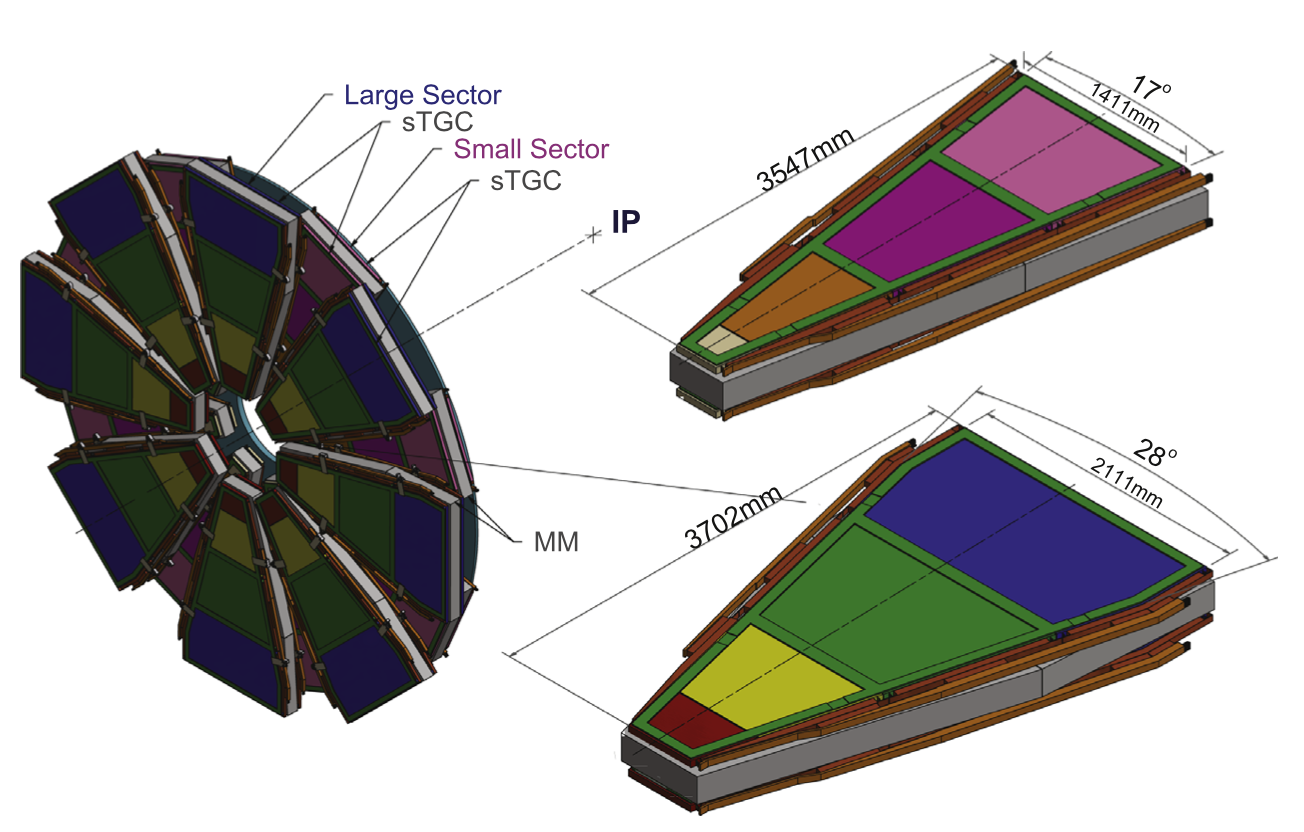
\includegraphics[width=0.7\textwidth]{NSW.png}
		\caption{New Small Wheel}\label{fig:nsw}
\end{figure}

The NSW will have two chamber technologies, one primarily devoted to the Level-1 trigger function (small-strip Thin Gap
Chambers, sTGC) and the other one dedicated to precision tracking (Micromegas detectors, MM). The sTGC are primarily deployed for
triggering given their single bunch crossing identification capability. The MM detectors have exceptional precision
tracking capabilities due to their small gap (\unit{5}{mm}) and strip pitch (approximately 0.5\si{mm}). Such a precision is
crucial to maintain the current ATLAS muon momentum resolution in the high background environment of the upgraded LHC.
The MM chambers can, at the same time, confirm the existence of track segments found by the muon end-cap middle
station (Big Wheels) online. The sTGC also has the ability to measure offline muon tracks with good precision, so the
sTGC-MM chamber technology combination forms a fully redundant detector system for triggering and tracking both for
online and offline functions. This detector combination has been designed to be able to provide excellent
performance for the eventual High Luminosity LHC upgrade.\par 



\section{sTGC Description}

The small-Strip Thin Gap Chamber (a.k.a sTGC) is a multi-wire proportional chamber (MWPC), a detector type
with a relatively old technology, its successful introduction to detector systems in 1968, it gave the Nobel prize to
George Charpak in 1992.  Those devices have been a major ingredient to detector systems since they can achieve spatial
resolution of several microns, and have typical time resolution of about 50ns.  The sTGC has been design to exploit
these features,  working with a cathode-anode pitch smaller than the anode-anode pitch, mostly based on the design of
the Thin Gap Chamber\cite{tgc}, with thinner strips as the main improvement from the previous version. The TGC technology
has been used since 1988 in OPAL experiment and is currently part of the muon spectrometer in ATLAS. \par
This new chamber has the advantage of having a \unit{3.2}{mm} strip-pitch (\unit{2.7}{mm} strips and \unit{0.5}{mm} gap) compare
to the \unit{6}{mm} from the previous TGC, which explains the {\it small-strip} prefix.\par
Chambers with different strips sizes were built and tested under pion beams, and the \unit{3.2}{mm} was chosen as the best
option\cite{stripwidth} to provide a resolution better than \unit{100}{\micro m}. 
This change will improve the
measurement of charge centroid position by charge interpolation.\par
To improve the time response, the cathode surface
resistivity has been reduced by a factor 10, to reduce charge accumulations on the cathode when chamber operates at
high rate, lowering from 1 M$\Omega/\square$ to 100-200k$\Omega / \square$ resistivity on the graphite layer.  At the
same time, cathode-readout plane (strips or pads) distance was reduced to \unit{0.1}{mm}(\unit{1.6}{mm} before) to
increase the capacitive coupling by 10, therefore the RC factor keeps unchanged.\par
%----------- sTGC mode picture -----

\begin{figure}[ht]
		\centering
		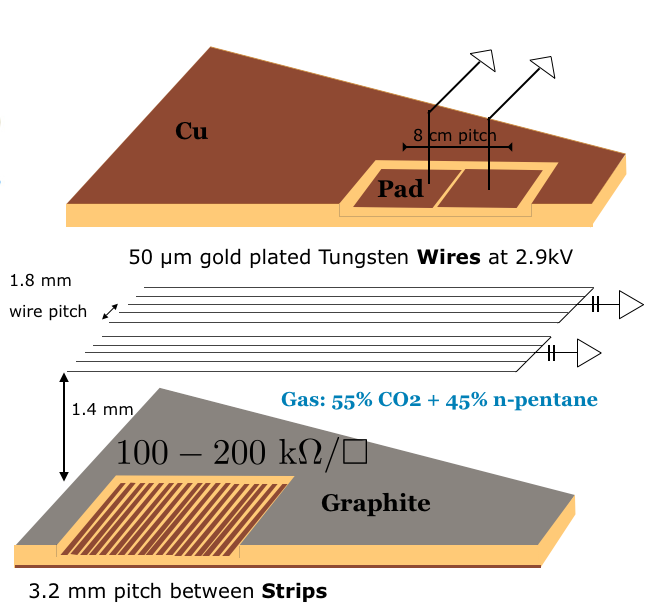
\includegraphics[width=0.5\textwidth]{sTGC_layout.png}
		\caption{Single plane sTGC}\label{fig:sTGC}
\end{figure}

The sTGC is made of two resistive cathodes planes, with copper readout plane with strips on one layer and the other one
with pads, with \unit{8x12}{cm$^2$} area used for fast pattern recognition of tracks to select strips for read out. This
represents a big
advantage compare to the TGC, which does not have this feature.\par
The cathodes are made of FR4 with \unit{1.6}{mm} of thickness, where \si{100}{\micro m} of copper is etched for strips
(pads), pressed with a \unit{100}{\micro m} of FR4 over it and then sprayed with graphite to provide superficial resistivity.\\
The anodes are golden tungsten wires of \unit{50}{\micro m} diameter,
distributed at \unit{1.8}{mm} between each other and a gas gap of \unit{2.8}{mm}. To work with such geometry, several
tests were made to find the proper gas
mixture\cite{gaschoice}. The most suitable mixture has been found to be 55\% of the well known carbon dioxide(CO$_2$)
as a quenching gas as a primary ingredient and 45\% of n-pentane(n-C$_5$H$_{12}$), which allow it to work in a limited
proportional region\cite{driftbook}(see Section 1.2.3). 
The latest ingredient; n-pentane, can absorb UV photons due to its many molecules degree of freedom,
hence it prevent the chamber going into a Geiger mode.\par 

%----------- How its produce the ionization and drifts  -----



\subsection{Electric field simulation}

Motivated by gaining better understanding of the detector operational mechanisms, dedicated simulations studies using
gaseous detector simulation tools have been performed. The main simulation tool used is Garfield
\cite{garfield2,garfield1} software package. This set of libraries allow to calculate the electrical field with
geometrical configuration as drift chambers.\par
The simulation uses a coordinate system where x is along the strips, y defines the chamber depth and z is along the
wires.\par

\begin{figure}[ht]
	\centering
	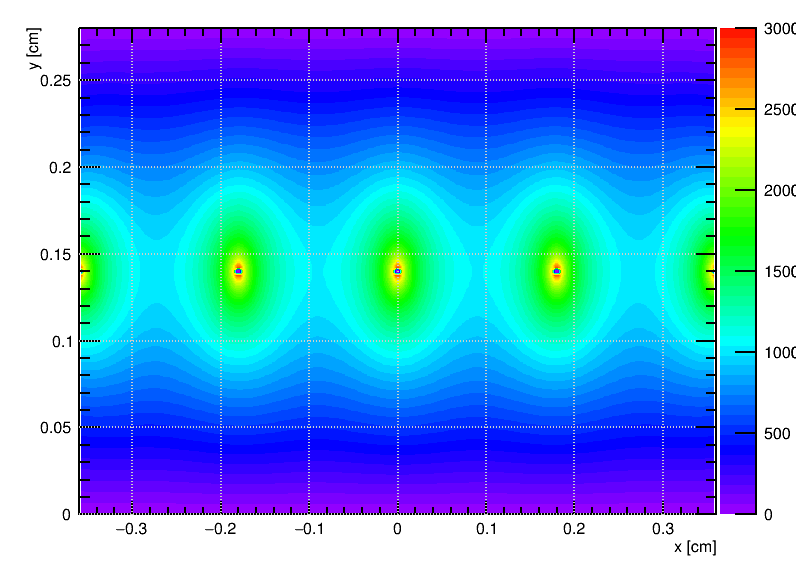
\includegraphics[width=0.5\textwidth]{vfield.png}
	\caption{Equipontential lines, anode at 2900V}\label{fig:vfield}
\end{figure}

\begin{figure}[ht]
		\centering
		\hspace*{\fill}
		\begin{subfigure}[b]{0.45\textwidth}
			\centering
			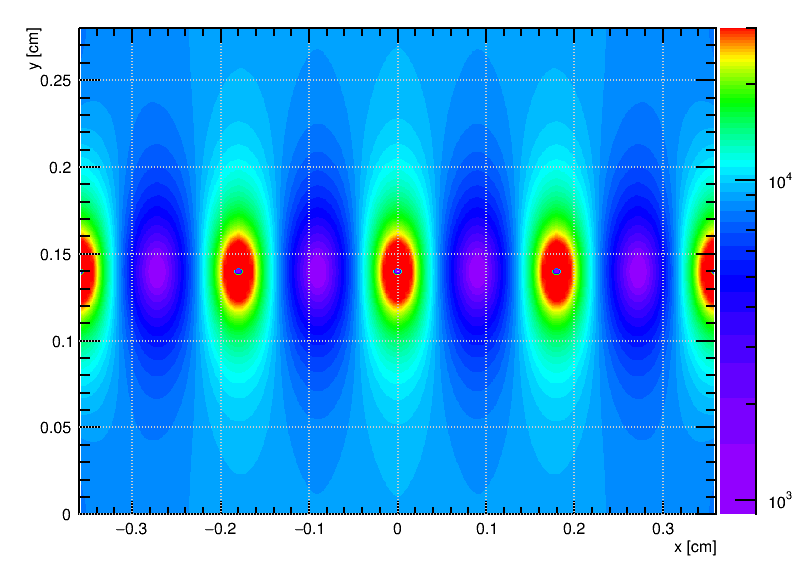
\includegraphics[width=\textwidth]{25efield.png}
			\caption{Electrical field, anodes at 2500V}\label{fig:25efield}
		\end{subfigure}
		\hfill
		\begin{subfigure}[b]{0.45\textwidth}
			\centering
			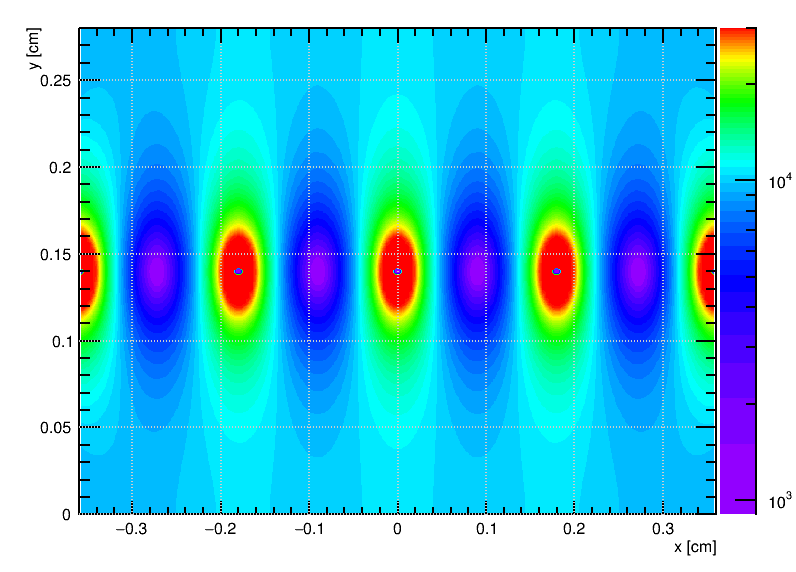
\includegraphics[width=\textwidth]{efield.png}
			\caption{Electrical field, anodes at 2900V}\label{fig:efield}
		\end{subfigure}
		\hspace*{\fill}
		\caption{The electric field map in the x-y plane for a typical operating high voltage 2900V and 2500V.}\label{fig:efields}
\end{figure}

Both contour plots on figure \ref{fig:efields} represent the magnitude of the electrical field with scale of
\SIrange{1e3}{1e5}{V/cm} with 50 steps. At the working potential \SI{2.9}{kV} it is possible to observed a field
strength of  more than \SI{1e4}{V/cm} over a 97\% of the gas gap. The weakest field it is only in a small region in the
middle of two neighboring wires.
\section{Construction process}

The main novelty on this detector is the high resolution obtained on x-axis due to the strip boards and the alignment
between each chamber to get precision about 50\micro m and 30\micro m respectively.\par 
It is important to discuss how
is possible to achieve those numbers. Everything relies on how well those chambers are built and also how the cathodes
boards (strips and pads) are fabricated.\par The size of each chamber varies from \SIrange{0.7}{2}{m^2} with around 1m long,
where over 300-400 strips must be etched with a precision of 50\micro m. A standard length for PCB boards is \SI{70}{cm}.
Extremely precautions must be taken to provide the precision and parallelism between each strips, in one of the biggest PCB board ever made.\par 
The attempt of this sections is to
give an idea of how the sTGC Quadruplets are built, mostly on the first module 0 produced by UTFSM, which is the QS1
(Quadruplet Small sector, part 1).  Being the smallest detector to be produced for the NSW has some pros and cons. The
main cons is related to the position of the QS1 inside the NSW, it is the closest one to the interaction point and as
such, it gets the highest rate of particles. For the same reason, the position resolution is a key point and
the high efficiency response under a high rate environment is a must.\par
Some pros are related to its size, with approximately \SI{1.3}{m} long, \SI{35}{cm} the small base and 75cm the large one of the trapezoidal shape, the sTGC QS1 can be handled without any
problems during its construction.\par

\subsubsection{Quality Control of cathode boards}

The cathodes for the module 0 were made by an Italian company MDT, and since it was the first production, the review was
done on-site.\\
The thickness of the board is measured in 19 points around the perimeter with a micrometer. The
values of theses measurements must be within 1.4mm$\pm$25\micro m. Exceeding this numbers leads to the partial rejection
of the cathode boards, however if there is a single point deviation of less than 35\micro m from the average, it
could be used in combination with another cathode board that does not have the same local deviation. The raw data is
found in appendix X.\par An electrical test is done with a multimeter, to check if there is any short circuit between strips or
pads depending on the cathode board.\par
The last step and the most important is the dimensional control; it is performed on a granite table, with 2 pins that match the brass inserts
on the cathode and a special caliper. 
An Aluminum-ruler machined (see figure \ref{fig:ruler}) with a precision of 30\micro m at 20 Celsius
degrees is used as caliper.  Above the cathode board the misalignment is measured. The caliper is an
Aluminium ruler machining  with a precision of 30\micro m at 20 Celsius degrees, it has the same strip pitch for the first
and last five strips and to avoid any parallax the thickness is the edge for those strips is 1mm. Looking with a lens
glass around this point it possible to detect some misalignment between this two strips (caliper and cathode board). A
photography is taken and analyze to calculate this misalignment. For such distance (about 1 m long) some precaution must
be take, considering the expansion coefficient for both material.  Machining with a precision of 30\micro m measure at 20
Celsius degrees.\par

%------- Photography strip cathode board measurement ------------ % 
\begin{figure}[ht]
	\centering
	\hspace*{\fill}
	{\begin{subfigure}[b]{0.35\textwidth}
		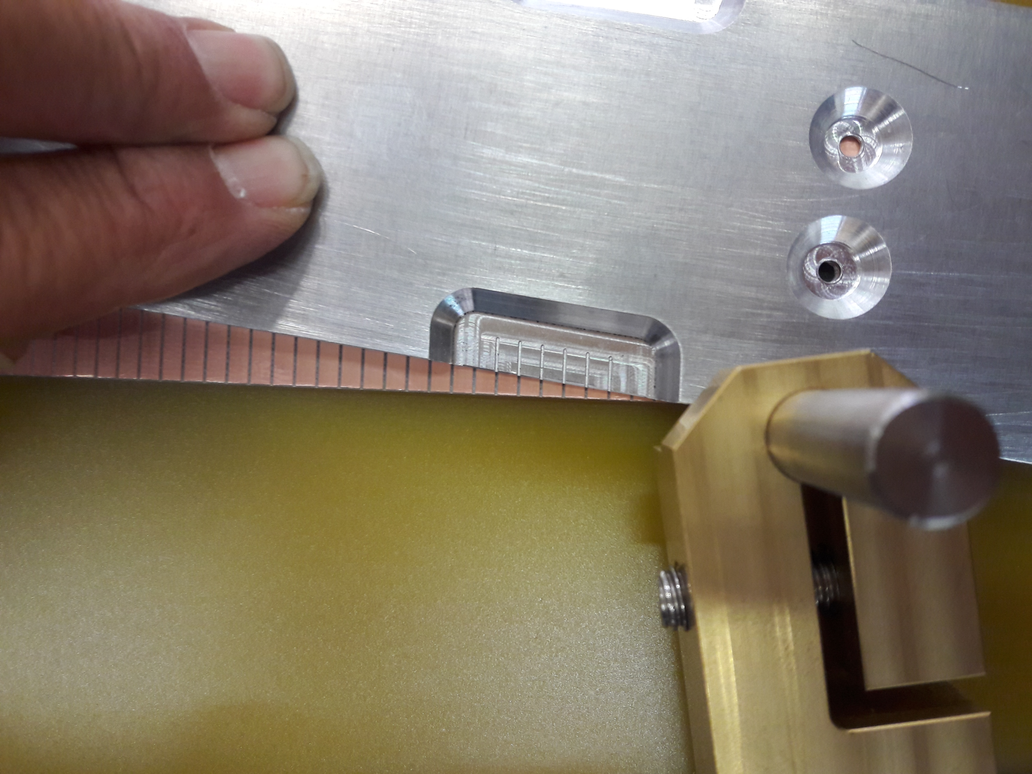
\includegraphics[width=\textwidth]{alignment.png}
		\caption{Al-ruler used to check shift over the last strips.}
		\label{fig:ruler}
	\end{subfigure}
	}
	\hfill
	{\begin{subfigure}[b]{0.35\textwidth}
		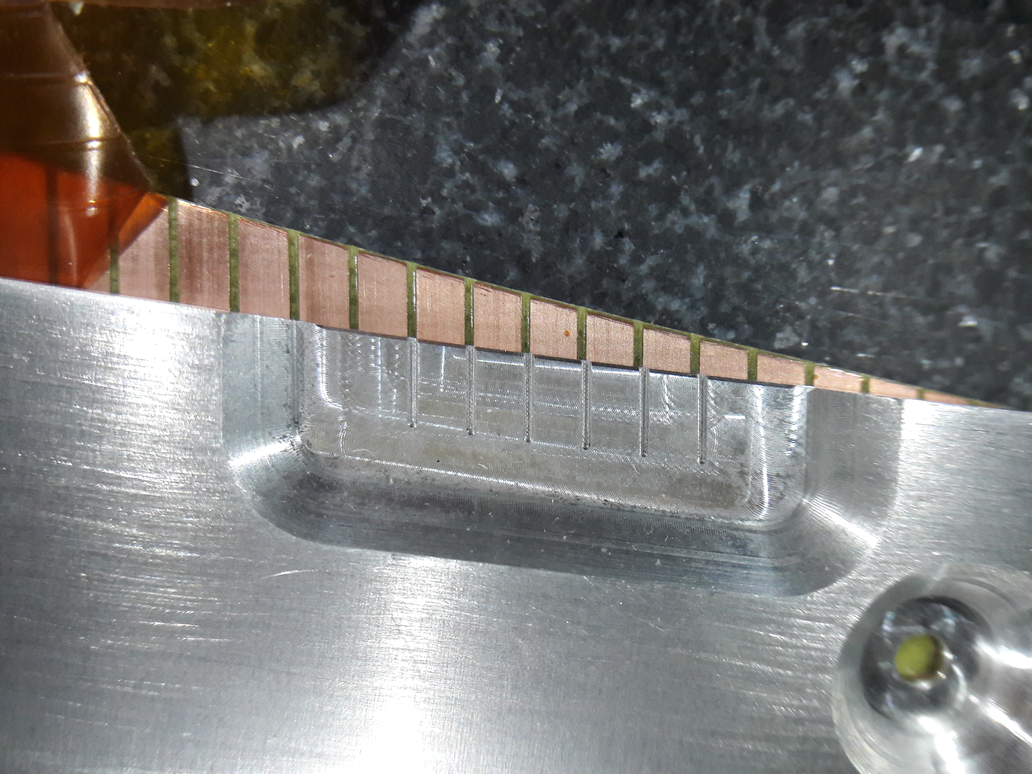
\includegraphics[width=\textwidth]{zoom_in.png}
		\caption{Zoom-in Comparing strip position}
		\label{fig:zoom}
	\end{subfigure}
	}
	\hspace*{\fill}
	\caption{Strip control with {\bf Al} caliper}
\end{figure}

\subsubsection{Cathode preparation}
Once the cathodes pass all the dimensional control, those had to be cleaned with Acetone and Isopropyl alcohol and placed on a
granite table (with a flatness  better than 30\micro m) with a vacuum system underneath. They have to be fixed on the edges with
metal jigs which have marks for the internal wire support or chamber division.\par
The places which are not sprayed with graphite, like the wire support and the edges, are covered with a \unit{3.5}{mm}
black tape on the designated wire support locations across the board. To prevent spraying graphite on the places where
there will be glue a blue tape must be placed on the edges.

\subsubsection{Graphite spraying}
A key point for this process is to prepare the ``painting", a mixture of Graphite-33 with Plastik-70 bonding agent. The
graphite must be agitated for at least 2 hours before mixing with Plastik-70. A proper ratio of 1500g Graphite and 540g
Plastik is mixed during 2 hours before spraying. The mixture must be is continuing mixing while \par
A spraying machine is in charge of this process, and meanwhile
temperature and humidity must be controlled. 
After the cathode is painted, the superficial resistivity is measured on the
edges. Values must exceed \unit{100}{k$\Omega/\square$} otherwise the cathode needs to be sprayed again.\par


\subsubsection{Polishing}
In order to ensure an uniform resistivity across the chamber, the cathode is visually divided in to 5x6 sections. Inside
each section, the resistivity is measured on 5 to 7 points with a probe. Simultaneously the cathode is brushed in the
same orientation as the wires. The brush must be done carefully, without over-polishing areas, since once resistance
drops down, nothing will bring it back up. 


\subsubsection{Glue internal parts}
After removing all the blue and black tapes, all the internal parts (buttons, wire support, etc. are glued to provide mechanical support to the gas gap.\par
The wire support and the buttons help the chamber not to bend due to gravity and not to create a catenary effect.
The external frames provide the \unit{1.4}{mm} height for the gas gap. 
All these part are cleaned with isopropyl alcohol, 
While the glue, a type of epoxy (2011-Araldite) is prepared, all these parts are cleaned with isopropyl alcohol.
This glue will not only fix the parts, it will also fill the surfaces where these parts are less thick than requested.


\subsubsection{Winding wires}
A flat table which can spin around one axis is used to wind the cathodes board.
On each side of the table, one cathode with all the internal parts is tight with metal clamps on
the edges.
At the same time, vacuum is applied underneath to ensure the flatness of the cathode. 
A winding machine places each wire at \unit{1.8}{mm} distance from each other with
\unit{50}{\micro m} precision.\\ 
After the process is completed, all the wires are soldered in batches of 10
over the wire-rulers with \unit{10}{M$\Omega$} resistor to the high voltage line.
Later on, the remaining wire can be cuted and the metal clamps around the edges can be removed. 

\subsubsection{Detector Assembly}

Once the cathodes are winded and all wires are soldered, the Pad cathode board is cleaned with clean water and dried with clean air.
The board is placed on the granite table (with vacuum underneath) to be tested with high voltage.
It is necessary to monitor the current from the cathode while the voltage is increased.
It starts with 100V and reaches 3000V, with steps of  100V.  The current should never reach a value higher than
\unit{1}{\micro A}. If it does, the cathode needs to be checked carefully, to remove dust or glue which create sparkles.\\ 
Reaching the nominal current, the strip cathode board is placed against the pad cathode board
carefully.
An Aluminium frame with a silicon rubber is placed on top to isolate the chamber from the environment.
Afterwards, vacuum is applied to this chamber and only CO$_2$ is flushing inside the chamber.\par
The power supply is turned on and no sparkles (monitoring the current) must be found.\par
In order to prevent dust entering the chamber the glue is prepared to close the chamber immediately.
Upon completion of the process, a single chamber is built.\par
A doublet is assembled with two single chamber glued with a honeycomb paper. Repeating the process with two doublets,
the quadruplet is built.
\begin{figure}[ht]
\centering
\hspace*{\fill}
{\begin{subfigure}[b]{0.55\textwidth}
\includegraphics[width=\textwidth]{quadreal.png}
\caption{Module \#0 against alignment pin}\label{}
\end{subfigure}
}\hfill
{\begin{subfigure}[b]{0.35\textwidth}
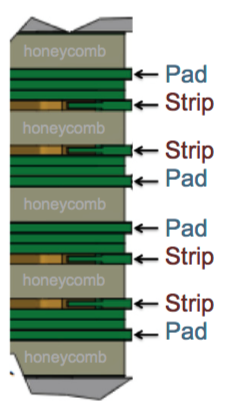
\includegraphics[height=7cm]{quadlayers.png}
\caption{Layer description}\label{quad}
\end{subfigure}
}\hspace*{\fill}
\caption{}
\end{figure}


\section{Gain uniformity measurements}

After the chambers are built, it is important to look for any malfunctioning. A primitive test to check the behavior of
the detector, is to use a radiation source and move it across the sensitive area and measure the current draw from the
power supply. This test will give us the first answer of the gain of our detector.\par
In this test, it is important to understand what can produce variation on the gain. There are two main ingredients that can produce gain variations on wire
detectors. The first one is the ``nature" gain fluctuations from the charge production in proportional counters which
follow Polya distribution, however is less pronounced in limited-proportional mode such as sTGC working region.\\
The second one is related to the mechanical tolerances, this part is very well known since 40 years as it is presented on
Sauli's book \cite{sauli} about drift chambers and tell us:
\begin{itemize}
\item A diameter variations of the wire about 1\% (fabrication precision) will result on a 3\% change in the gain.
\item  \unit{100}{\micro m} difference in the gas gap thickness(\unit{2.7}{mm}) results in about 15\% change on the gain.
\item The effect of a wire displacement of about \unit{100}{$\mu$m}
of a wire plane results in 1\% in the charge of the two adjacent wires which with a gain of $\sim10^6$ will give a
$\sim10\%$ change on the gain.
\end{itemize}
Taking all of this in consideration, it is expected to get a gain variation less than 20\% according to the
Construction manual\cite{mann}.\par

The amount of current measured from the power supply it will be considered as gain reference, while the detector is
irradiated with x-rays. The test is performed under two different working points (bias voltage), 2500V (low gain) and
2900V, the operational voltage.\par

%-------- why x ray source ? ----------
For such test the x-ray source is used thanks to the advantages:\par
\begin{itemize}[noitemsep, topsep=0pt, parsep=0pt, partopsep=2pt]
	\item Mostly mono-energetic photons.
	\item Variable photon intensity: Limiting the current from the tube from \SIrange{1}{200}{\micro A} can provides different rates.
	\item Variable photon energy: Varying the breaking voltage of electrons inside the x-ray gun from
	\SIrange{10}{50}{kV}.
	\item Different spot size: with a set of collimator it is possible to irradiate only interesting area.
\end{itemize}


\subsection{Setup}
To perform such test, a x-ray gun called Mini-X\cite{xgun} from Amptek is used, with silver (Ag) as transmission target and with a
beryllium (Be) end-window is used.\par

\begin{figure}
	\centering
	\hspace*{\fill}
	{\begin{subfigure}[b]{0.4\textwidth}
	\centering
	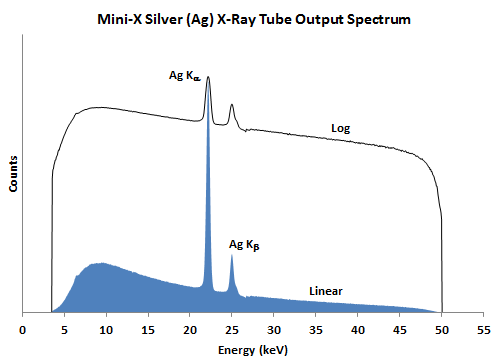
\includegraphics[width=\textwidth]{minix_ag_1.png}
	\caption{Output spectrum, from 0 to 50keV}\label{fig:minixgun}
	\end{subfigure}
	}
	\hfill
	{
	\begin{subfigure}[b]{0.4\textwidth}
	\centering
	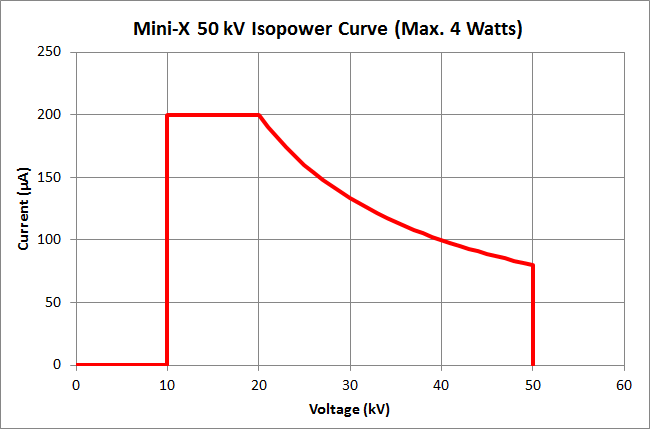
\includegraphics[width=\textwidth]{minix_d.png}
		\caption{Isopower curve for the Mini-x gun}\label{fig:ispower}
	\end{subfigure}
	}
	\hspace*{\fill}
	\caption{}\label{}
\end{figure}

\begin{figure}
	\centering
	\hspace*{\fill}
	{\begin{subfigure}[b]{0.4\textwidth}
	\centering
	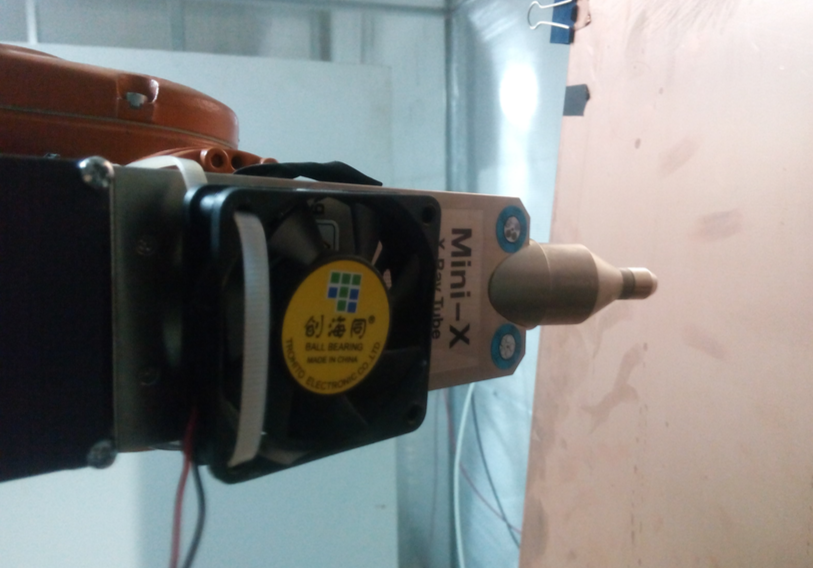
\includegraphics[width=\textwidth]{kuka.png}
	\caption{Mini-X gun mounted on KUKA robo-arm}\label{fig:kuka}
	\end{subfigure}
	}
	\hfill
	{
	\begin{subfigure}[b]{0.4\textwidth}
	\centering
	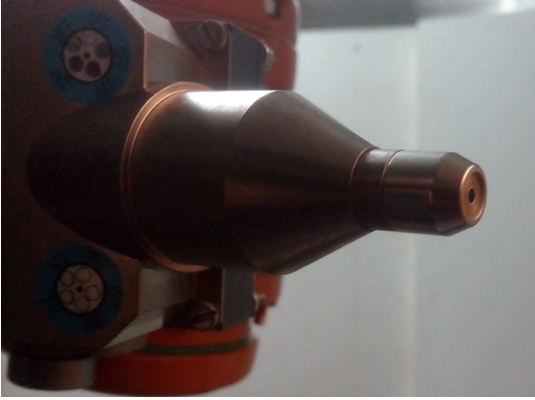
\includegraphics[width=\textwidth]{collimator.png}
		\caption{Collimator 2mm}\label{fig:collimator}
	\end{subfigure}
	}
	\hspace*{\fill}
	\caption{}\label{}
\end{figure}

The gun is mounted on a KUKA robo-arm (see Fig.\ref{fig:kuka}), with a 5 degrees collimator providing a \SI{4}{mm^2} spot size at a proper
distance. The robo-arm provide the x-y movement to scan the whole sensitive detector area, moving from the small base to
the large base along the wires at step of \SI{1.2}{cm/s}. Each y-movement were separated for \SI{5}{cm}, being not the
most suitable distance to irradiate the whole detector, but it was choose to work properly with the x-ray gun at
\SI{45}{\micro A}, 50keV energy (see figure \ref{fig:ispower}) without overheating the gun.\par
A NIM HV Power Supply Module CAEN 1470 was used to power the chambers. The power supply (PS) was controlled by USB with the
CAEN HV Wrapper Library. The current registered from the PS was written in a ASCII file for further analysis. The
sampling rate used from the PS was 1 per second, giving the current average during this period.\par

The test is taken in approximately one hour, irradiating one chamber at the time.\par
Since the detector is already built as a quadruplet, it has to turn over to irradiate the other face of it. Hence, only
the external layers (chambers) are irradiated directly without having an chamber to provide an screening effect.\par

\begin{figure}[ht]
	\centering
	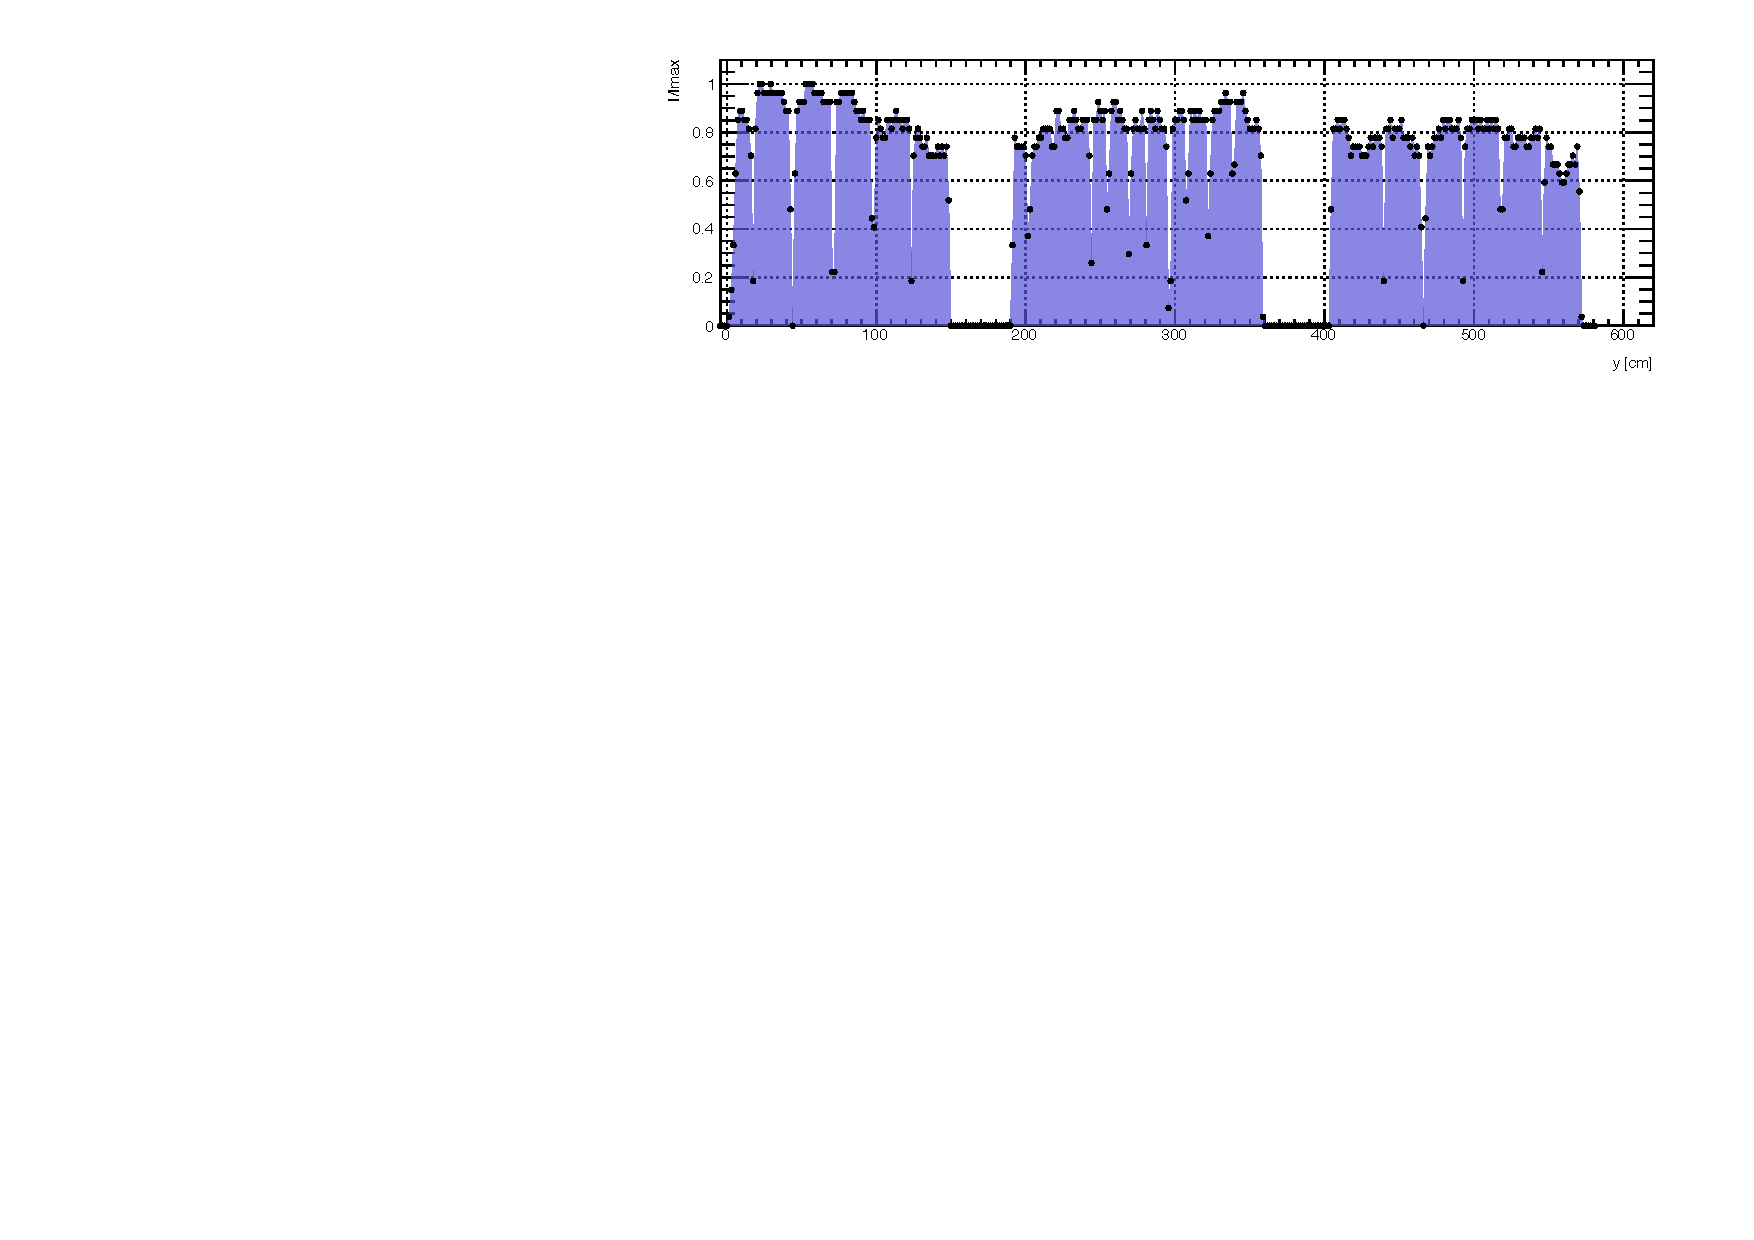
\includegraphics[width=\textwidth]{uniformity_2900.pdf}
	\caption{Relative current to the maximum, while the robo-arm is moved along the detector passing 3 times at different
	position across the wires (x-axis)}\label{}
\end{figure}


\subsection{Results}

\begin{figure}[ht]
	\centering
	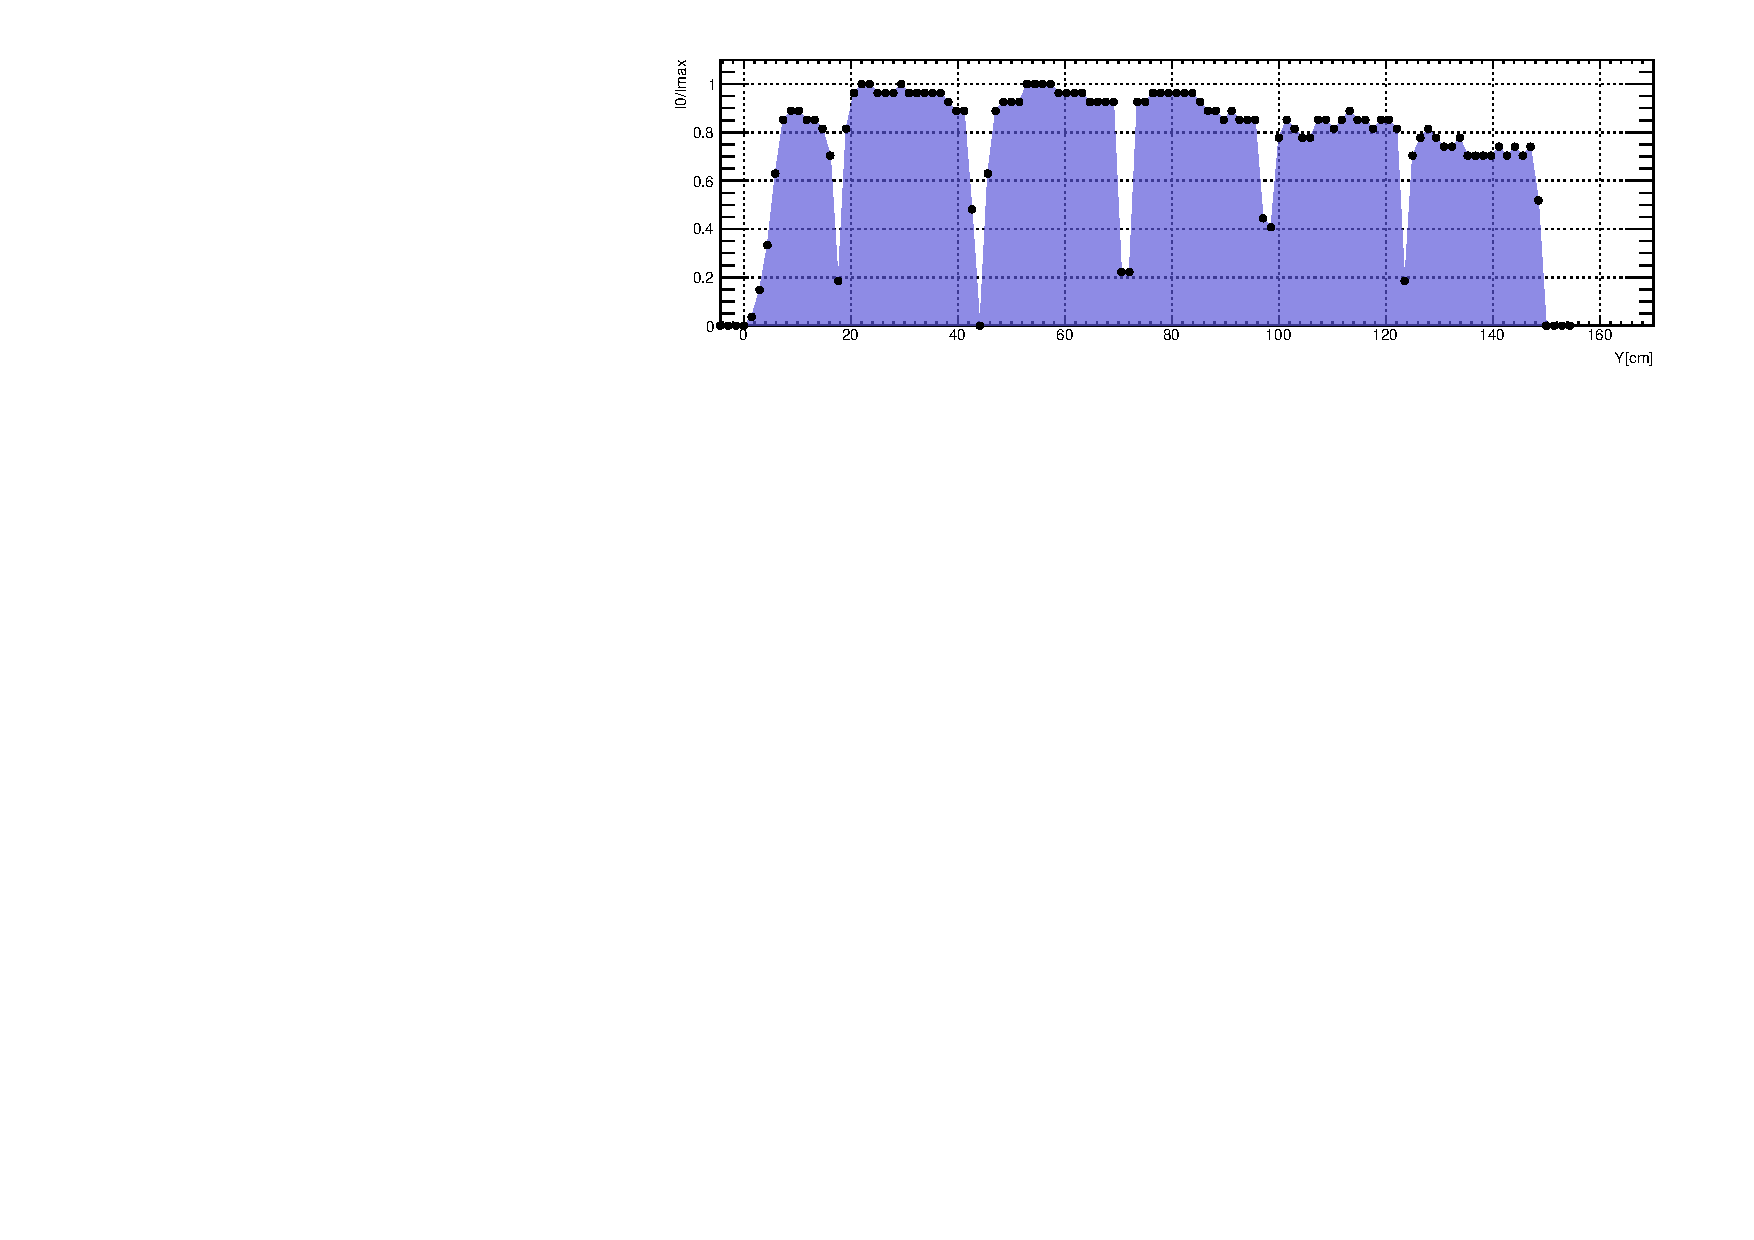
\includegraphics[width=\textwidth]{relativecurrent.pdf}
	\caption{Moving across strips, wire-supports are present with minimum gain.}\label{fig:structure}
\end{figure}

At first glance, it is possible to observed the internal structure of the chamber with this test. Looking the plot
\ref{fig:structure} the current decrease when the gun is irradiating the places where the wire-supports are found. In
theses places a small gas volume is present, therefore less electrons can drift to the wires, resulting in less current
draw from the power supply.\par
If a better meshing of the irradiation places can be perform, the identification of the wire-supports and the chamber
separation (small and large sector) can be obtained with good resolution, however, it can be obtained with this test, a
width of 
\SIrange{17}{23}{mm} of theses internal parts, when the real size is \SI{20}{mm}.\par

Interpolating the points (x, y, I) an overall picture can be obtained (figure \ref{fig:xyscan}). The figure shows a line
with high current resulting from a missing wire on the chamber 2. More charge is collected on the neighbors when a wire
missing, resulting from a longer drift path.\par


\begin{figure}[ht]
		\centering
		\hspace*{\fill}
		\begin{subfigure}[b]{0.45\textwidth}
			\centering
			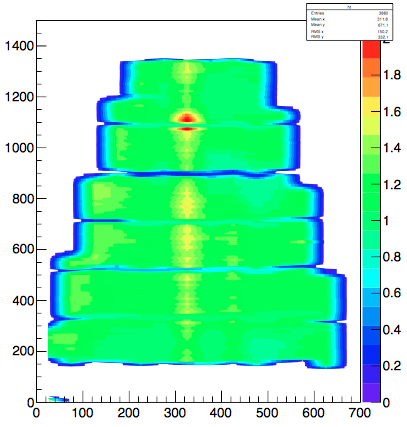
\includegraphics[width=\textwidth]{xy_scan.png}
			\caption{xy-scan chamber 2 sTGC Module \#0: missing wire}\label{fig:xyscan}
		\end{subfigure}
		\hfill
		\begin{subfigure}[b]{0.45\textwidth}
			\centering
			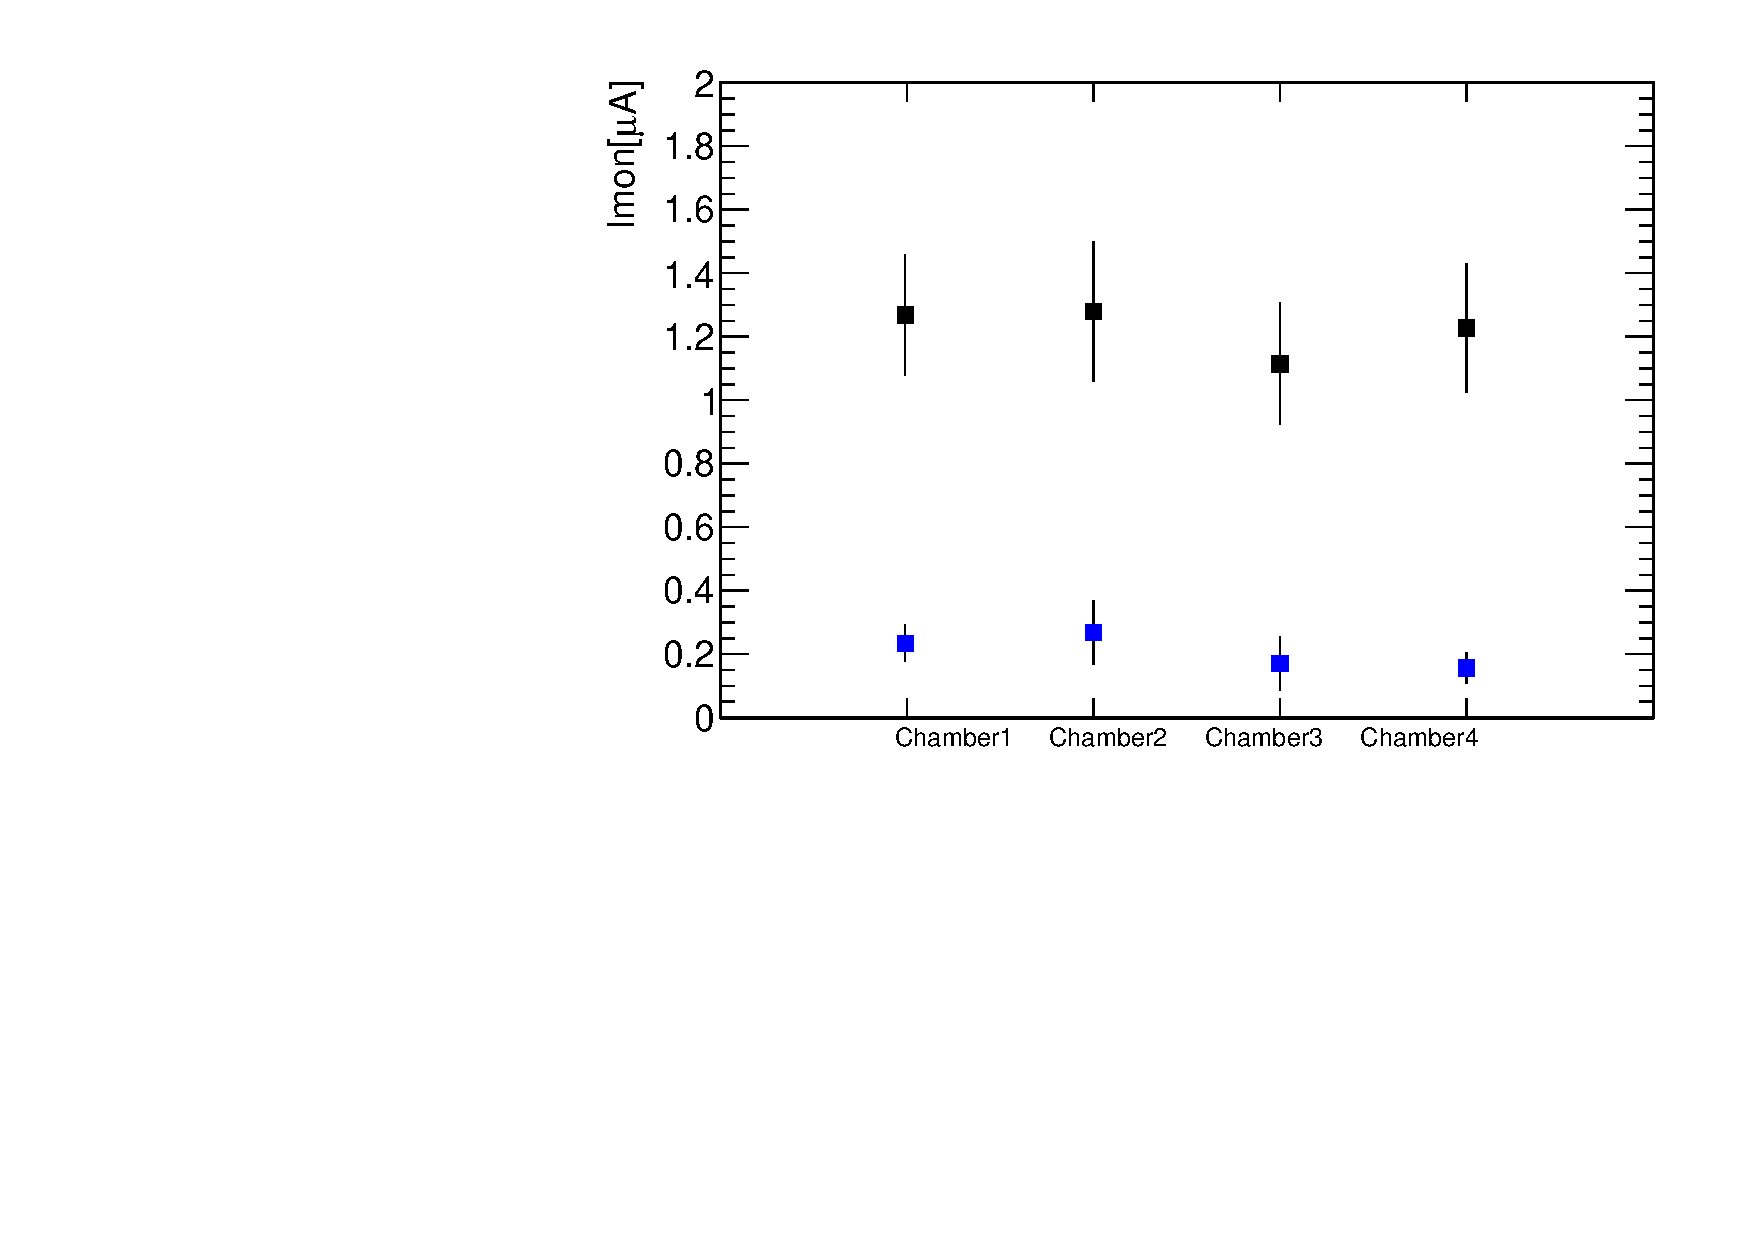
\includegraphics[width=\textwidth]{graphgain.pdf}
			\caption{Current draw at 2.5kV (blue) and 2.9kV(black)}\label{fig:draw}
		\end{subfigure}
		\hspace*{\fill}
		\caption{ }\label{}
\end{figure}


The graph on figure \ref{fig:draw} shows the average current from each chamber a two different working potential. The
average is calculated only for the sensitive area, hence the places where the wire-support are present are not part from
the average. The current on average at 2.5kV and 2.9kV are \SI{200}{nA} and \SI{1.2}{\micro A} respectively.\par 
%Considering the approximate flux \cite{xgun}, $\Phi_{Xray} =$ $10^6$ [phonts/s mm$^2$] at \SI{30}{cm} is possible
%to estimate the flux at 5cm with a current tube 45 times higher. 
%\begin{equation}
%\mathrm{\Phi_0 = 45 \cdot 25 \cdot \Phi_{Xray}(r=30cm)\sim 10^9 \left[ photons/s\cdot mm^2\right ]}
%\end{equation}


\begin{table}
	\centering
	\begin{tabular}{ccccc}
	\hline
	& Chamber 1&Chamber 2 & Chamber 3 & Chamber4\\
	$\sigma$/mean\% 	
	 & 15.08\%  
& 17.18\%  
	 & 17.25\%  
	& 16.64\%  \\
	\hline\\
	\end{tabular}
	\caption{Uniformity gain}\label{table}
\end{table}

The table \ref{table} summarize the uniformity obtained, calculated as the RMS over the mean from the current draw
distribution for each chamber. The four chambers have less than 20\% of gain variation, which it was expected from the
construction manual.\par



\section{Stability under high rate}

One of the key feature of this detector is that must be able to work under high particles flow
rates (\unit{15}{kHz/cm$^2$}), and the first step is
check either the device or its electronic components can handle this high rate.\par
\begin{figure}[ht]
	\hspace*{\fill}
	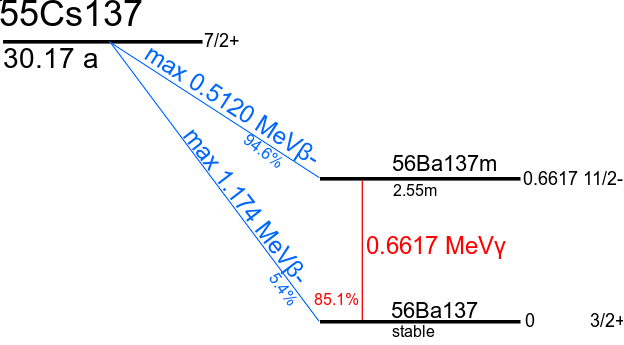
\includegraphics[width=0.5\textwidth]{cesiumdecay.png}
	\hspace*{\fill}
	\caption{Cesium-137 Decay scheme.}\label{cesium}
\end{figure}
\begin{figure}[ht]
	\hspace*{\fill}
	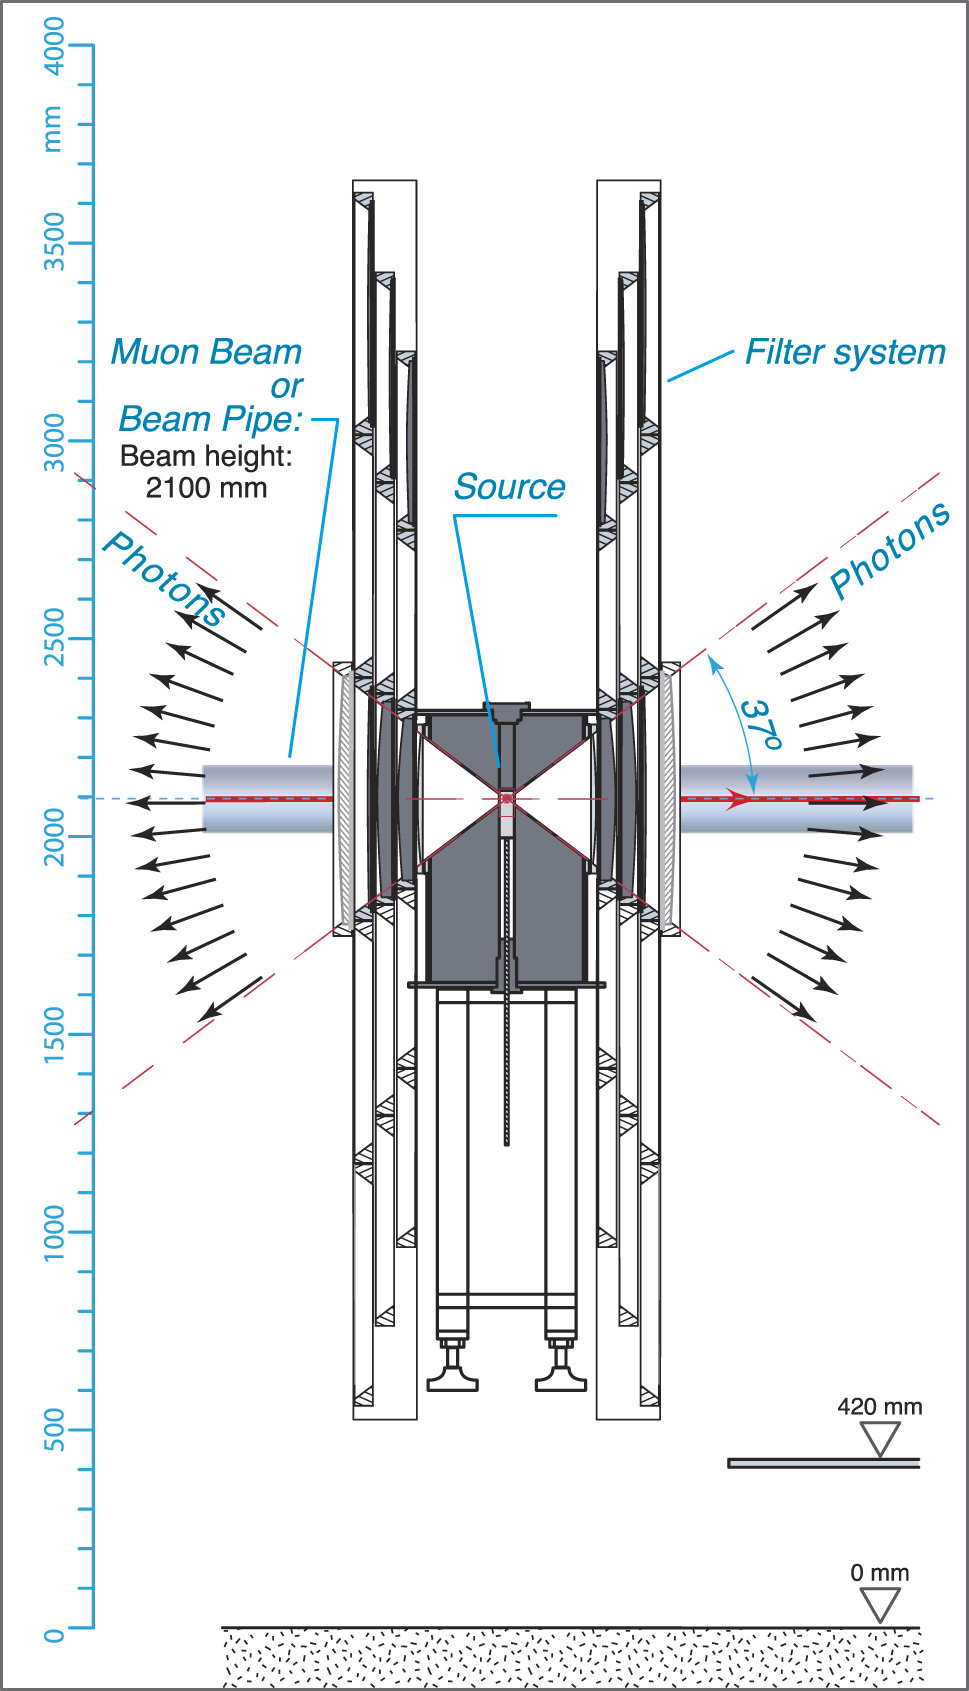
\includegraphics[width=0.4\textwidth]{filters.png}
	\hspace*{\fill}
	\caption{Irradiator with filter system. Three different rows with
		three lead (Pb) layer each one with different thickness helps to provide multiples rates for the facility.}\label{filters}
\end{figure}
For this purpose the module 0 was
	placed inside of a High Radiation Facility at CERN called GIF++\cite{gif}.
	The installation has a Cesium-137(Fig. \ref{cesium}) as a gamma source with an activity of approximately
	\unit{14.9}{TBq}(\unit{13.3}{TBq} during the test, August 2016). 
	A system of movable lead attenuators (figure \ref{filters}) for large irradiation zone, allows attenuation factors
	between 1 and $5\times10^5$
	in several steps.\par 
	In order to get the particle rate, a direct measurement setup was implemented with a  small size (\SI{16,2x12,4}{cm} as
	sensitive area) sTGC as a {\bf Monitor}. A LVDS (Low voltage differential signaling) logical signal from wires was obtained from an
	Amplifier Shaper Discriminator (ASD) board\cite{asdchip}. The ASD board provide the signal from 16 wires groups, all
	of them connected to a VME module (KEK ASD buffer) control the discrimator threshold from the ASD and convert the LVDS to NIM signal. The 16 LVDS signals are converted into
	two NIM logic signals. The two outputs from this modules are connected to an Scaler NIM n145 to provide the total rate
	on the {\bf Monitor}.\par

	The Module\#0 and the Monitor were placed at 1.3m distance from the source. Both connected in series to the same
	gas line, the temperature and pressure was recored to keep in track the working voltage, where most of the time the
	environmental conditions were 25 Celsius degree and \unit{971}{mb}.\\
	The working potential for the chamber is 2850V at \unit{1}{b}. Since the gain is proportional to $E/P$, the voltages
	must be increase in 2.9\% to correct de lower pressure, giving a 2935V as the new working point in this environment. 

	\begin{figure}[ht]
		\hspace*{\fill}
		\begin{subfigure}[b]{0.45\textwidth}
			\centering
			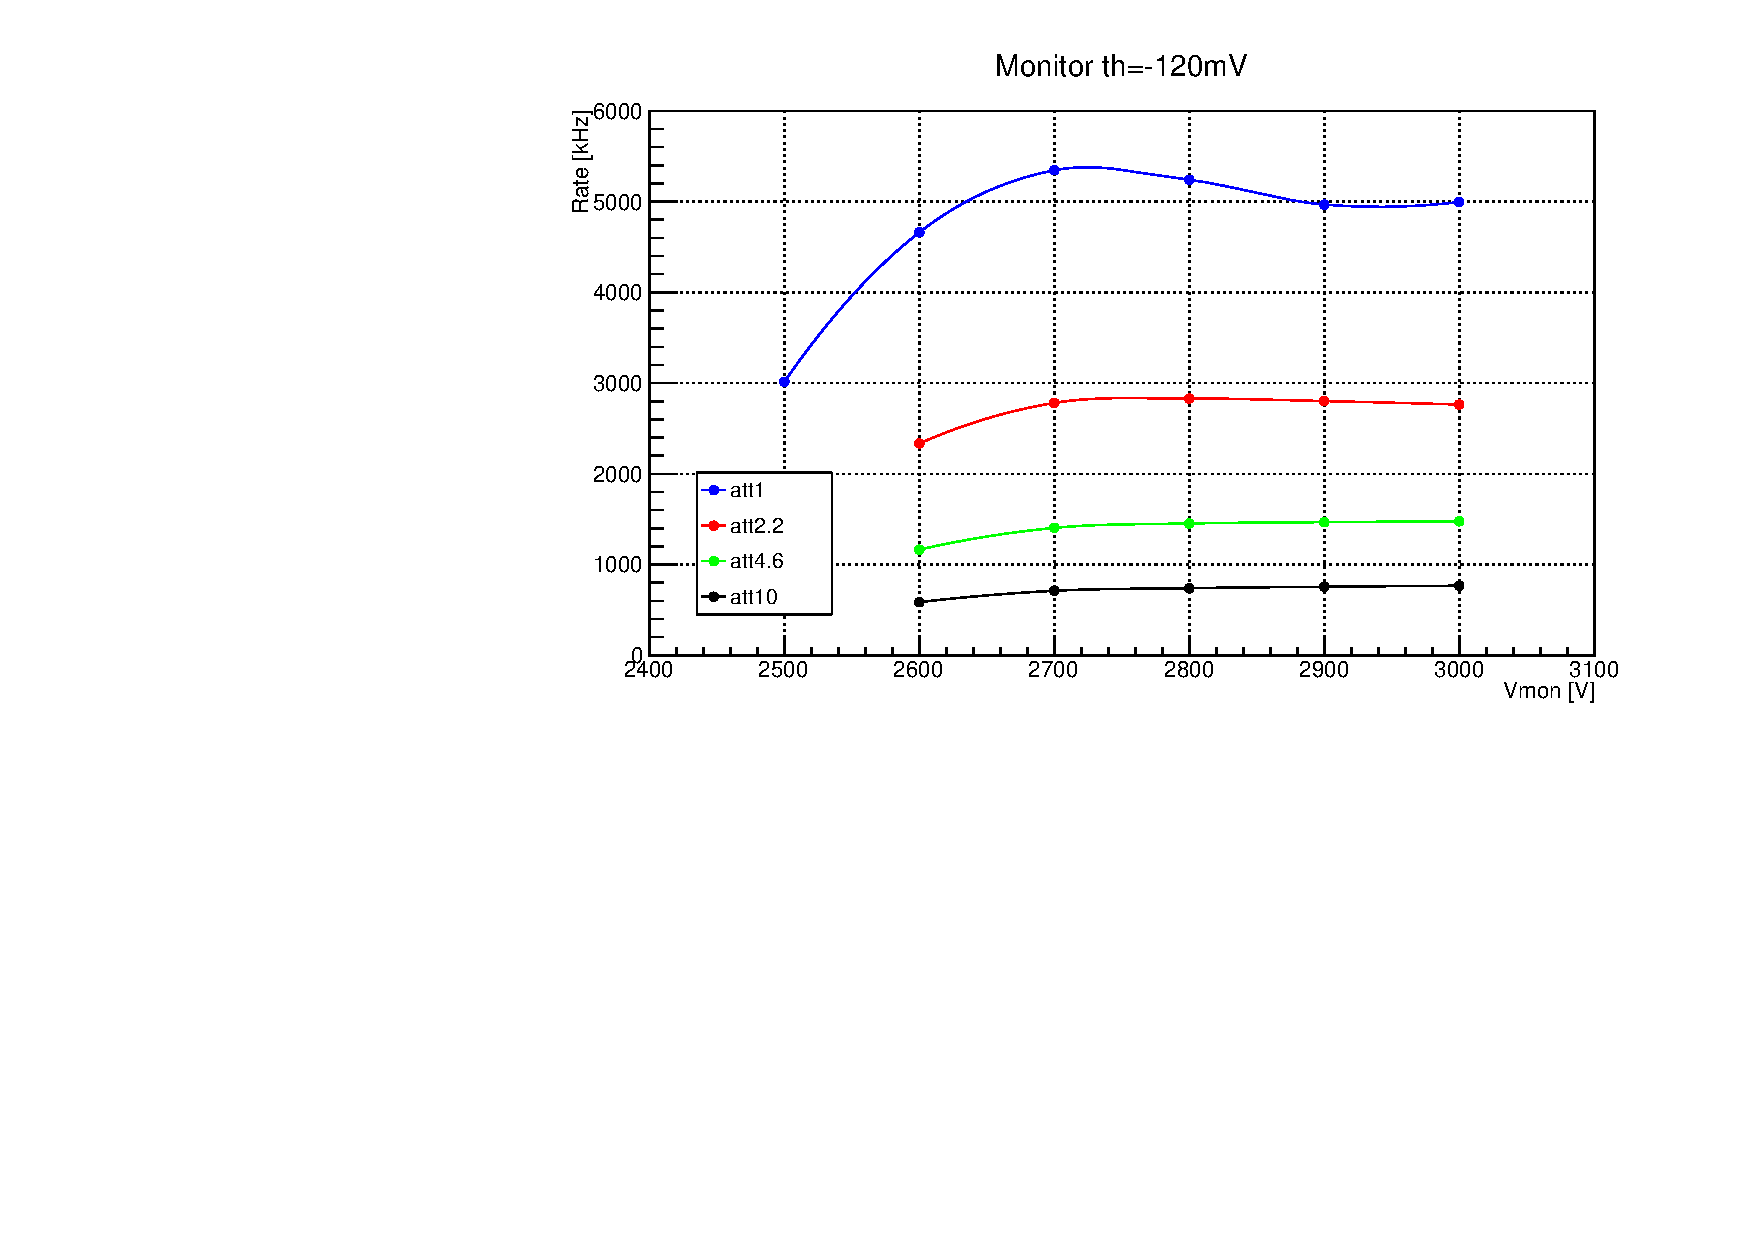
\includegraphics[width=\textwidth]{monitor.pdf}
			\caption{Different attenuation filters}\label{fig:monrate}
		\end{subfigure}
		\hfill
		\begin{subfigure}[b]{0.45\textwidth}
			\centering
			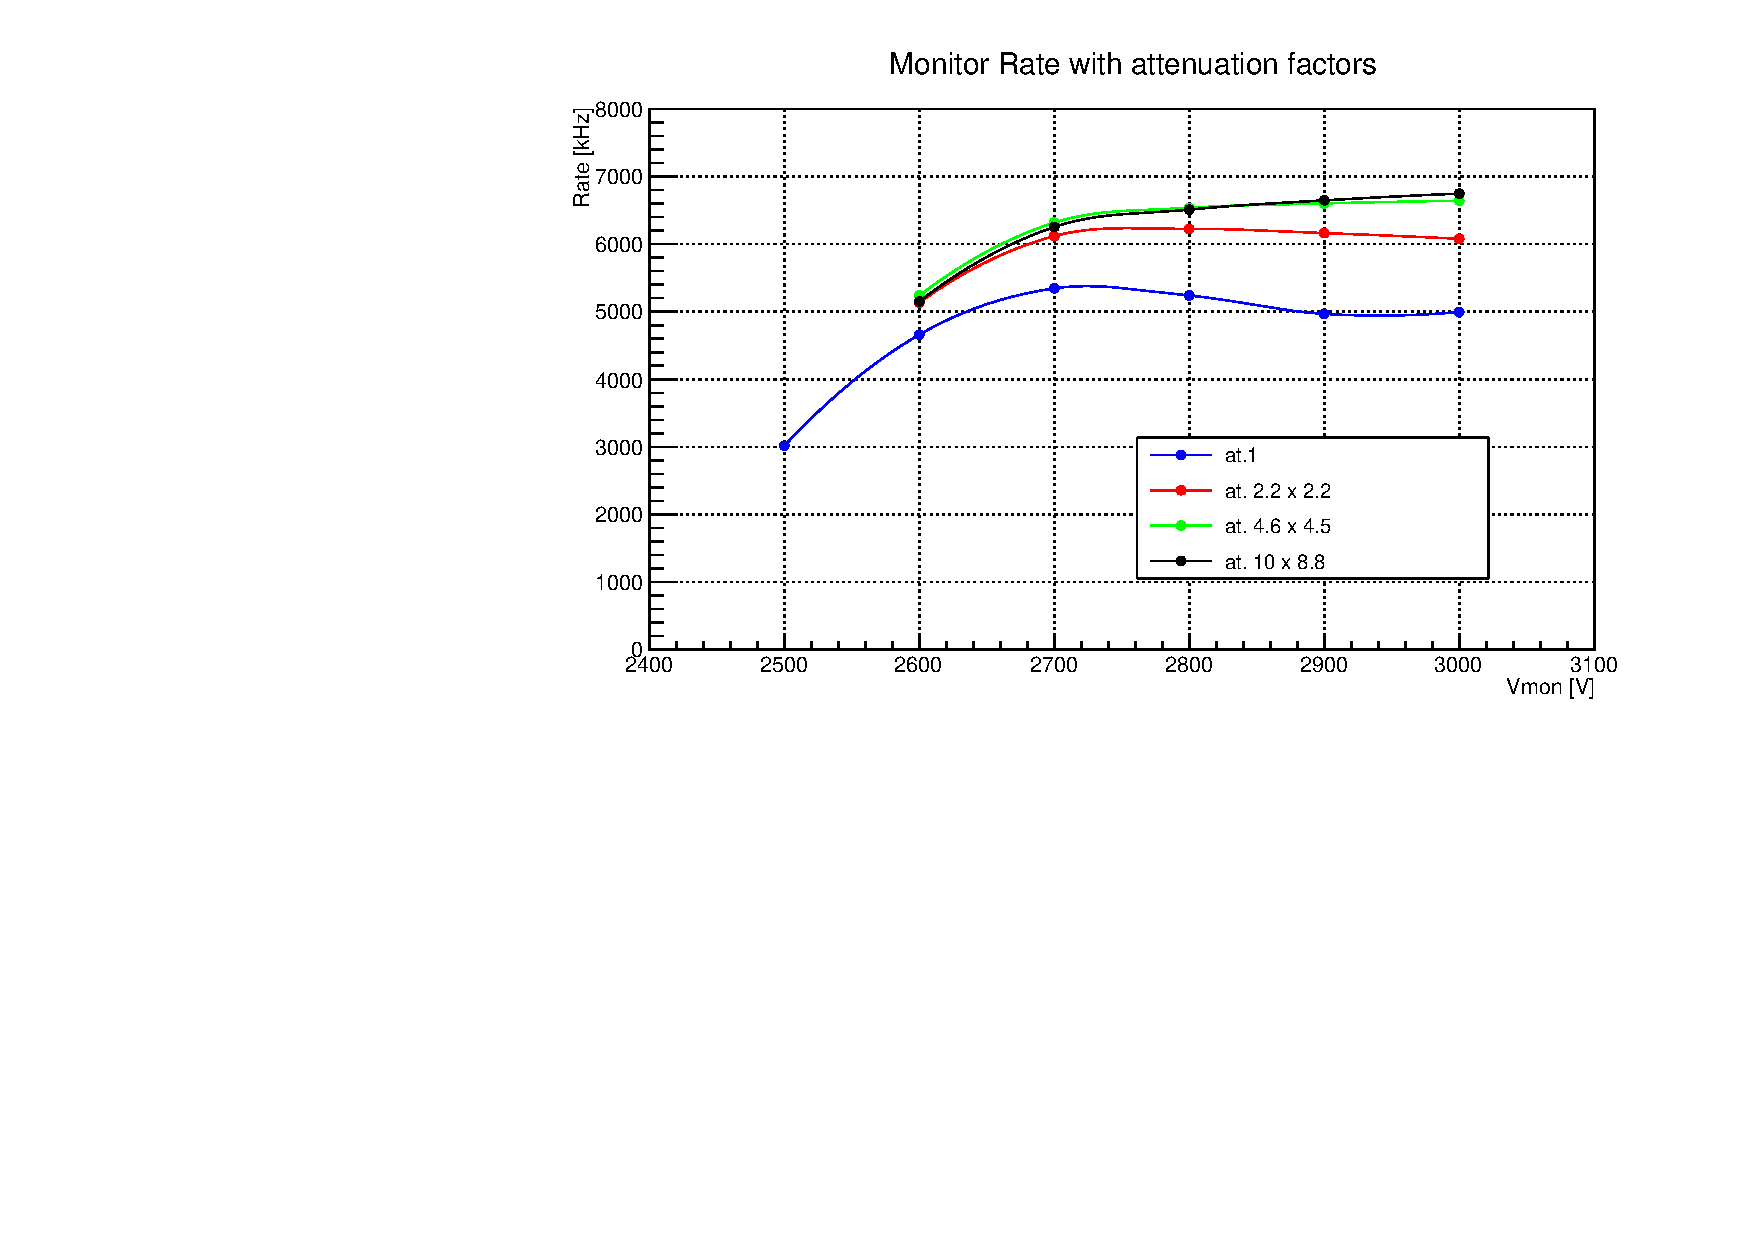
\includegraphics[width=\textwidth]{rate.pdf}
			\caption{Multiplying by att. Factors}\label{fig:filters}
		\end{subfigure}
		\hspace*{\fill}
		\caption{Rate on {\bf Monitor}}\label{}
	\end{figure}
	To achieve the background rate for ATLAS (\unit{15}{kHz/cm$^2$}), the Monitor must register more than \SI{2680}{kHz} if
	the sensitive area is considered. The sensitive area is calculated as the total area \SI{200}{cm^2} times the amount
	of wires group connected to the ASD (16 over 18).\par
	Four different attenuation factors were registered, where on Figure \ref{fig:monrate},
	is possible to observed two set of data over than the expected rate (red and blue). The other two set of data emphasizes the
	{\it plateau} reached over \SI{2.7}{kV}. At the same time, the highest rate shows an inefficiency on voltages over
	\SI{2.8}{kV} and the {\it plateau} is lost. Therefore, the data set with attenuation 2.2 (in red) is our reference.\par
	Multiplying the attenuation factors with each data set (Figure \ref{fig:filters}) will give us the expected rate with no
	filters, however, the data set with factor 1 has \SI{5}{MHz} at working potential, while the expected rate is
	\SI{6.6}{MHz}, resulting in an inefficiency of about 75\%. The flow rate recorded in this data set is \SI{28}{kHz/cm^2},
	almost the double than expected. At the same time, the interest should go on the red line (attenuation factor
	of 2.2) which represent the background level expected for ATLAS with an estimated flow rate of \SI{16.2}{kHz/cm^2} with
	an efficiency approximately of 93\% respect to the lowest rates.\par


	\begin{figure}[ht]
			\hspace*{\fill}
			\begin{subfigure}[b]{0.45\textwidth}
				\centering
				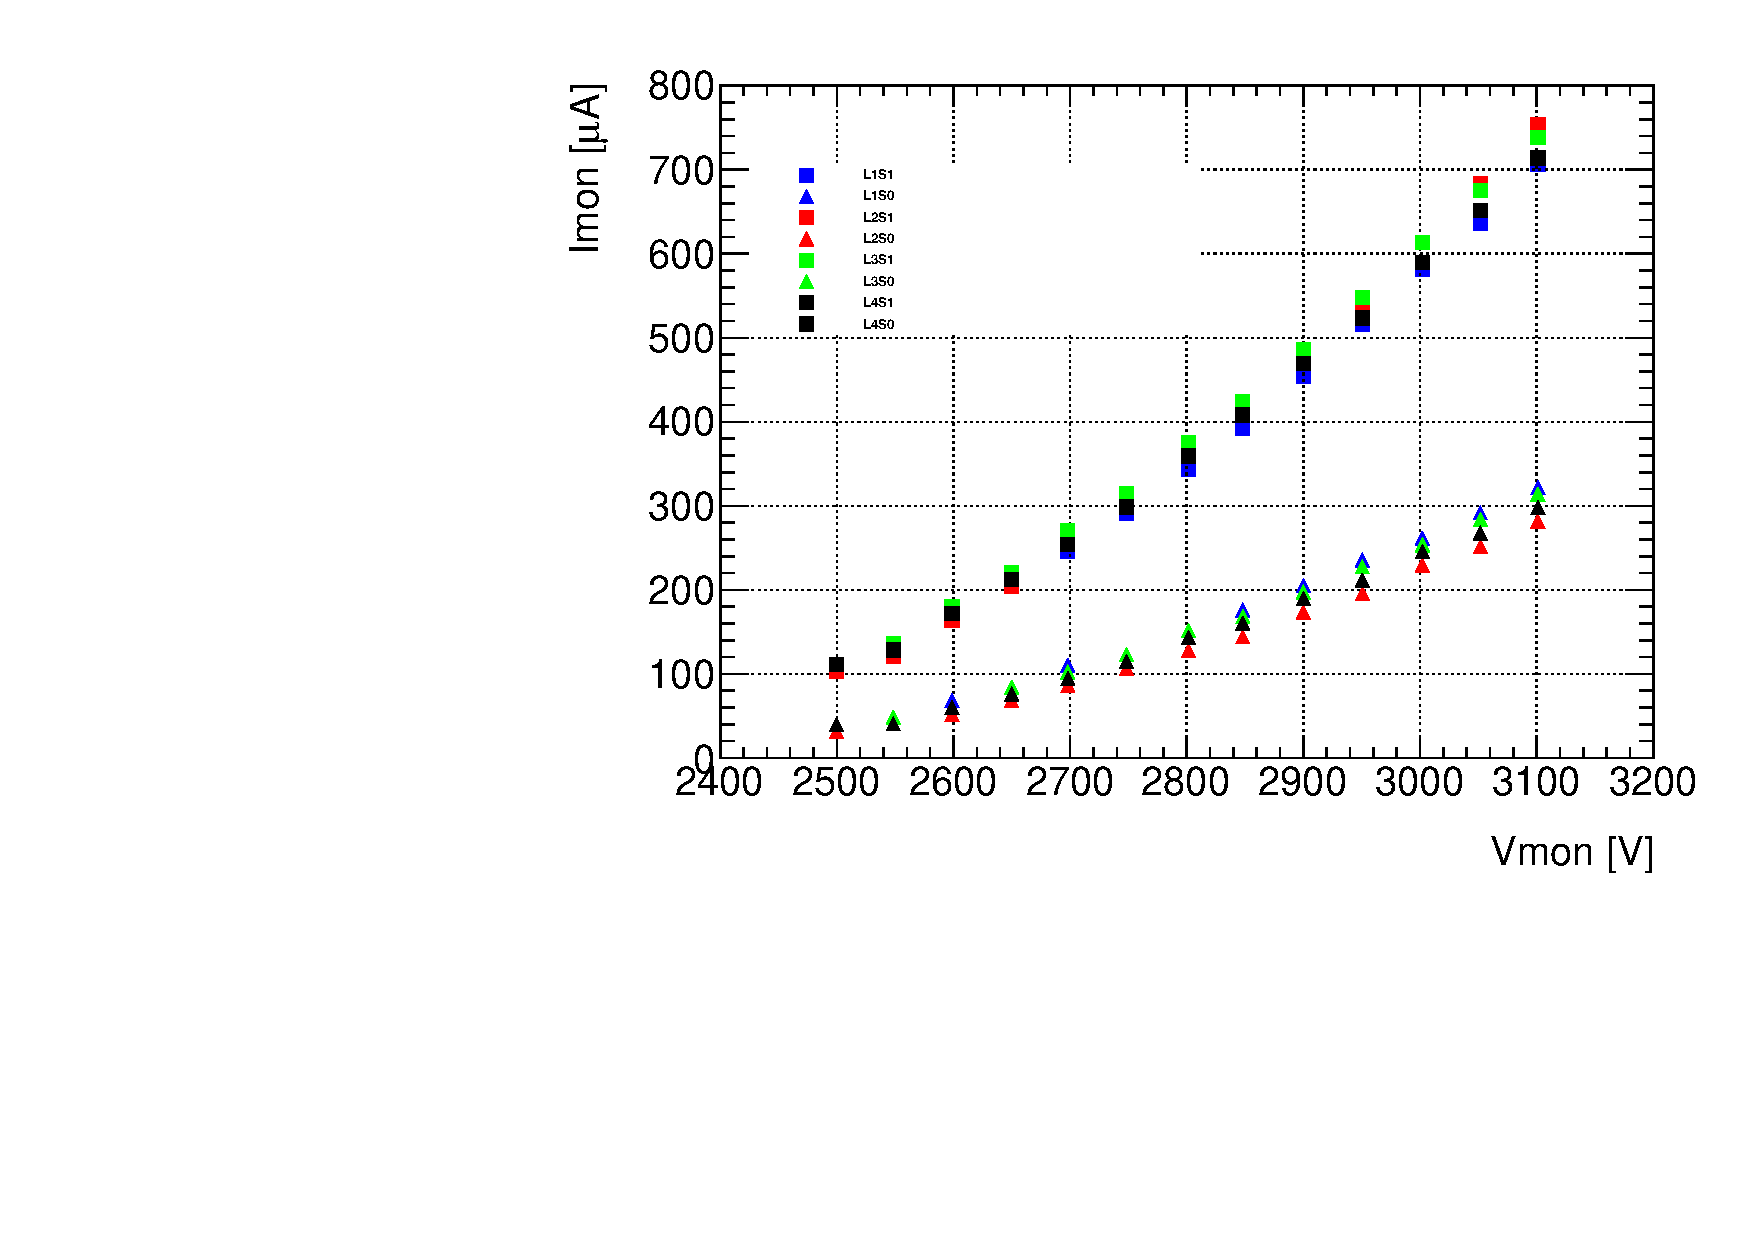
\includegraphics[width=\textwidth]{QS1_I_att1.pdf}
				\caption{Attenuation factor: 1}\label{fig:att1}
			\end{subfigure}
			\hfill
			\begin{subfigure}[b]{0.45\textwidth}
				\centering
				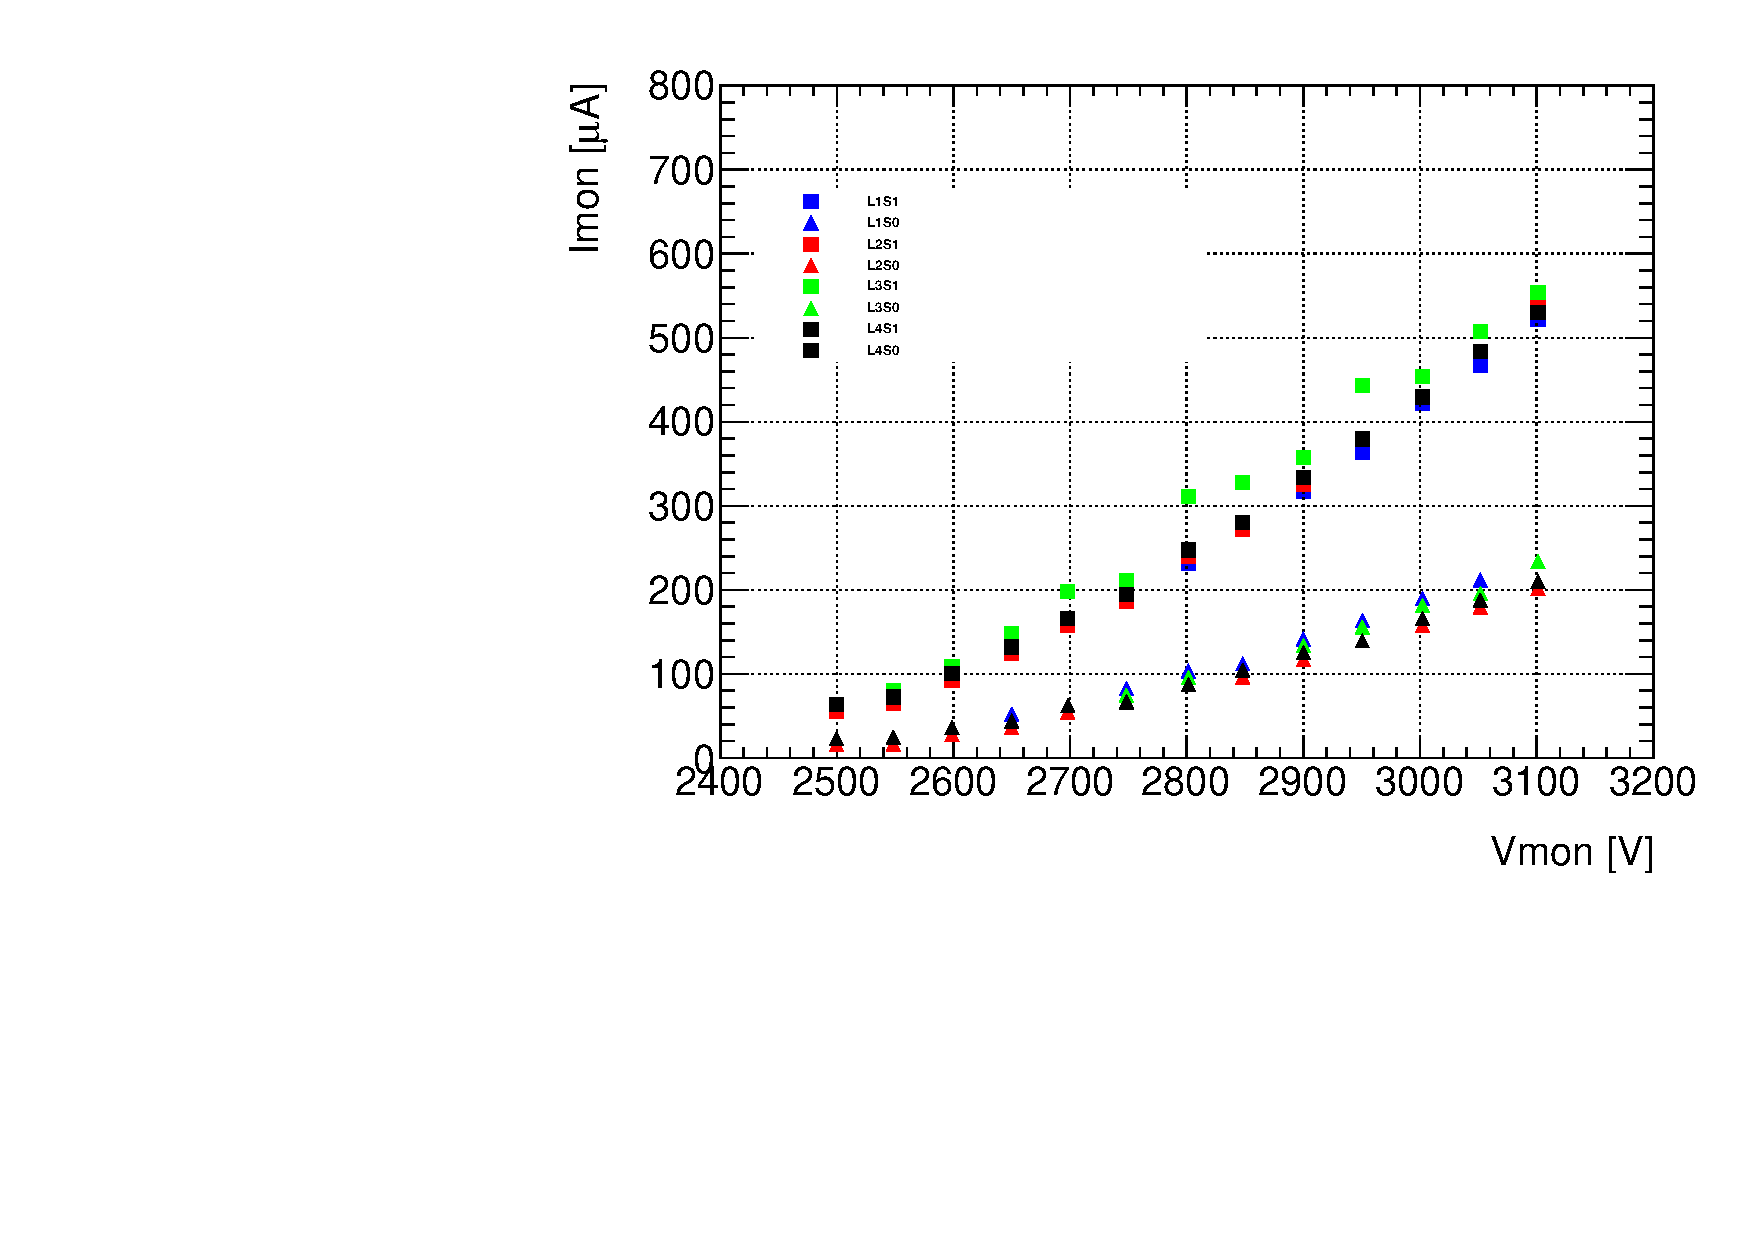
\includegraphics[width=\textwidth]{QS1_I_att22.pdf}
				\caption{Attenuation factor: 2.2}\label{fig:att22}
			\end{subfigure}
			\hspace*{\fill}\\
			\hspace*{\fill}
			\begin{subfigure}[b]{0.45\textwidth}
				\centering
				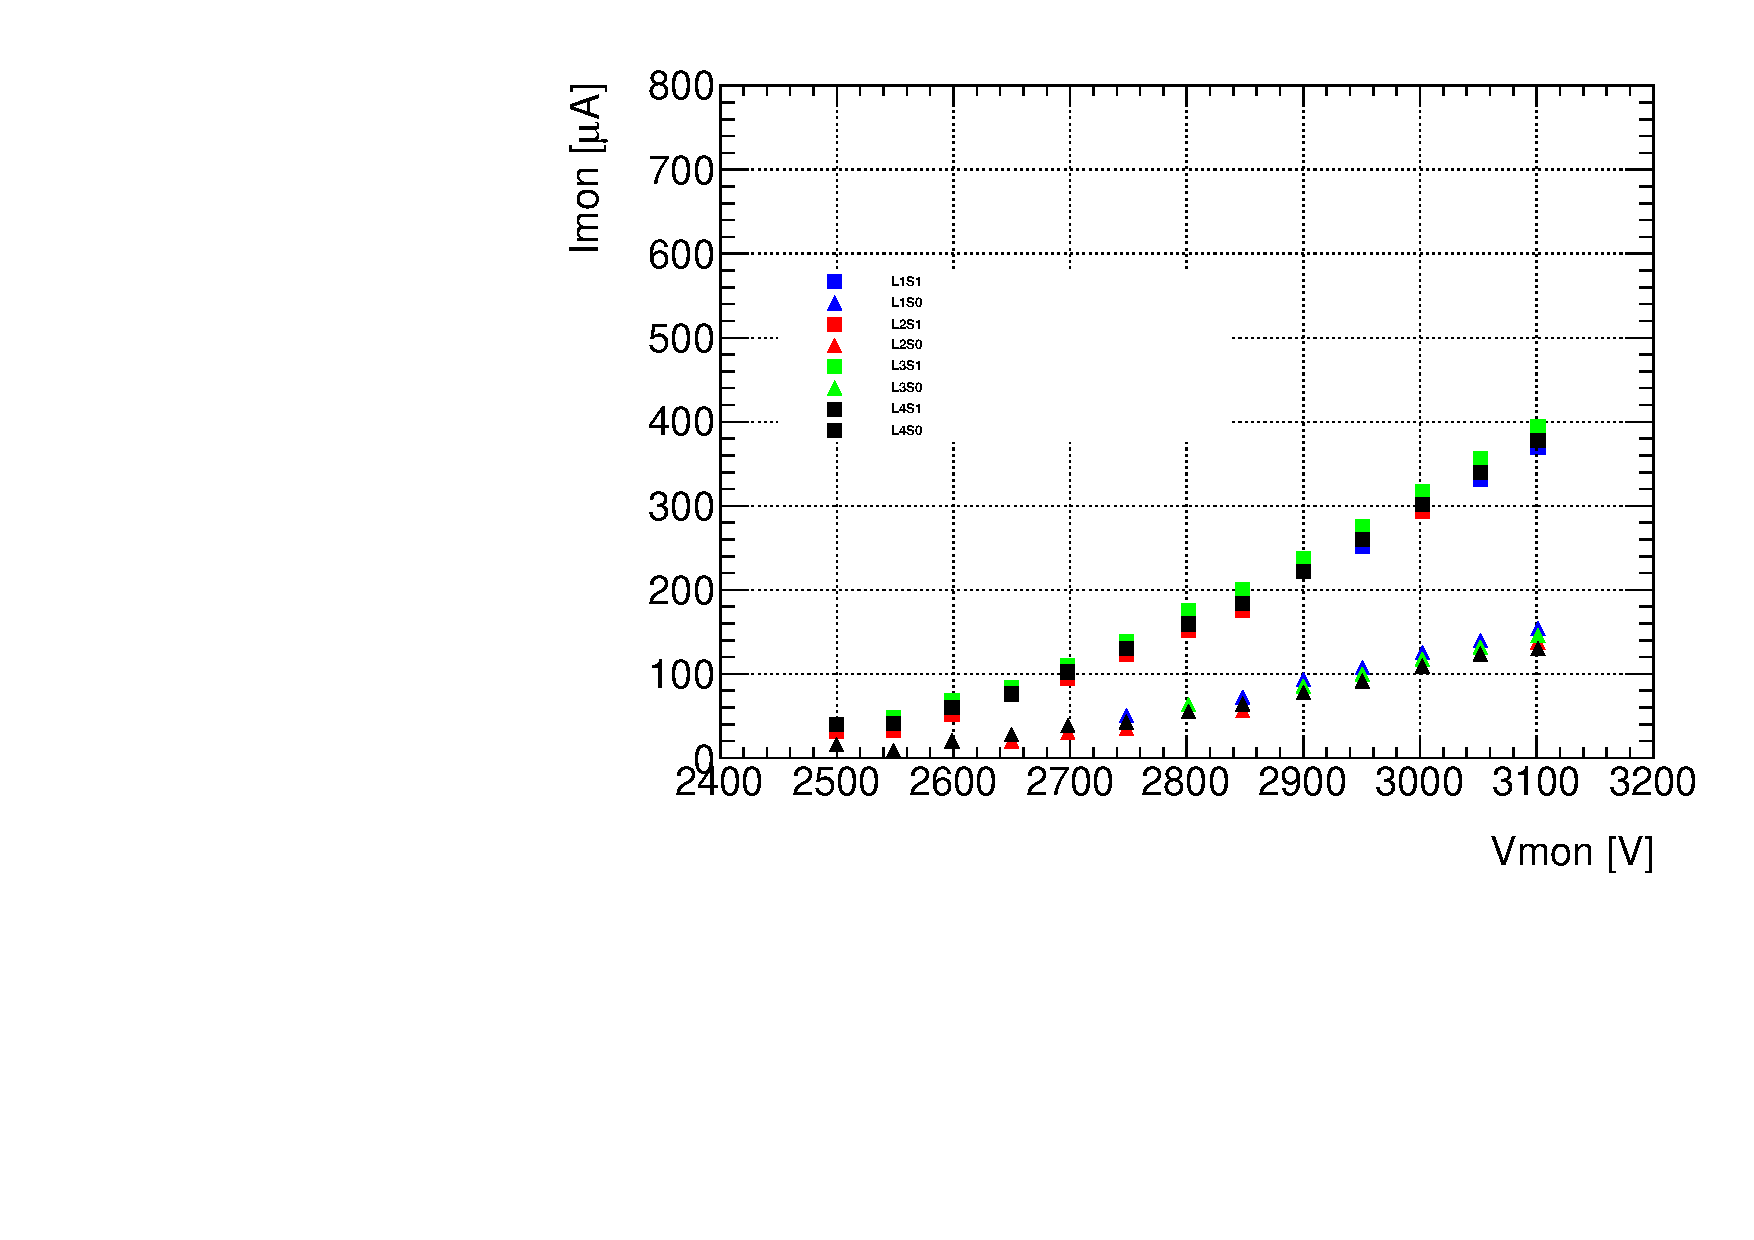
\includegraphics[width=\textwidth]{QS1_I_att46.pdf}
				\caption{Attenuation factor: 4.6}\label{fig:att46}
			\end{subfigure}
			\hfill
			\begin{subfigure}[b]{0.45\textwidth}
				\centering
				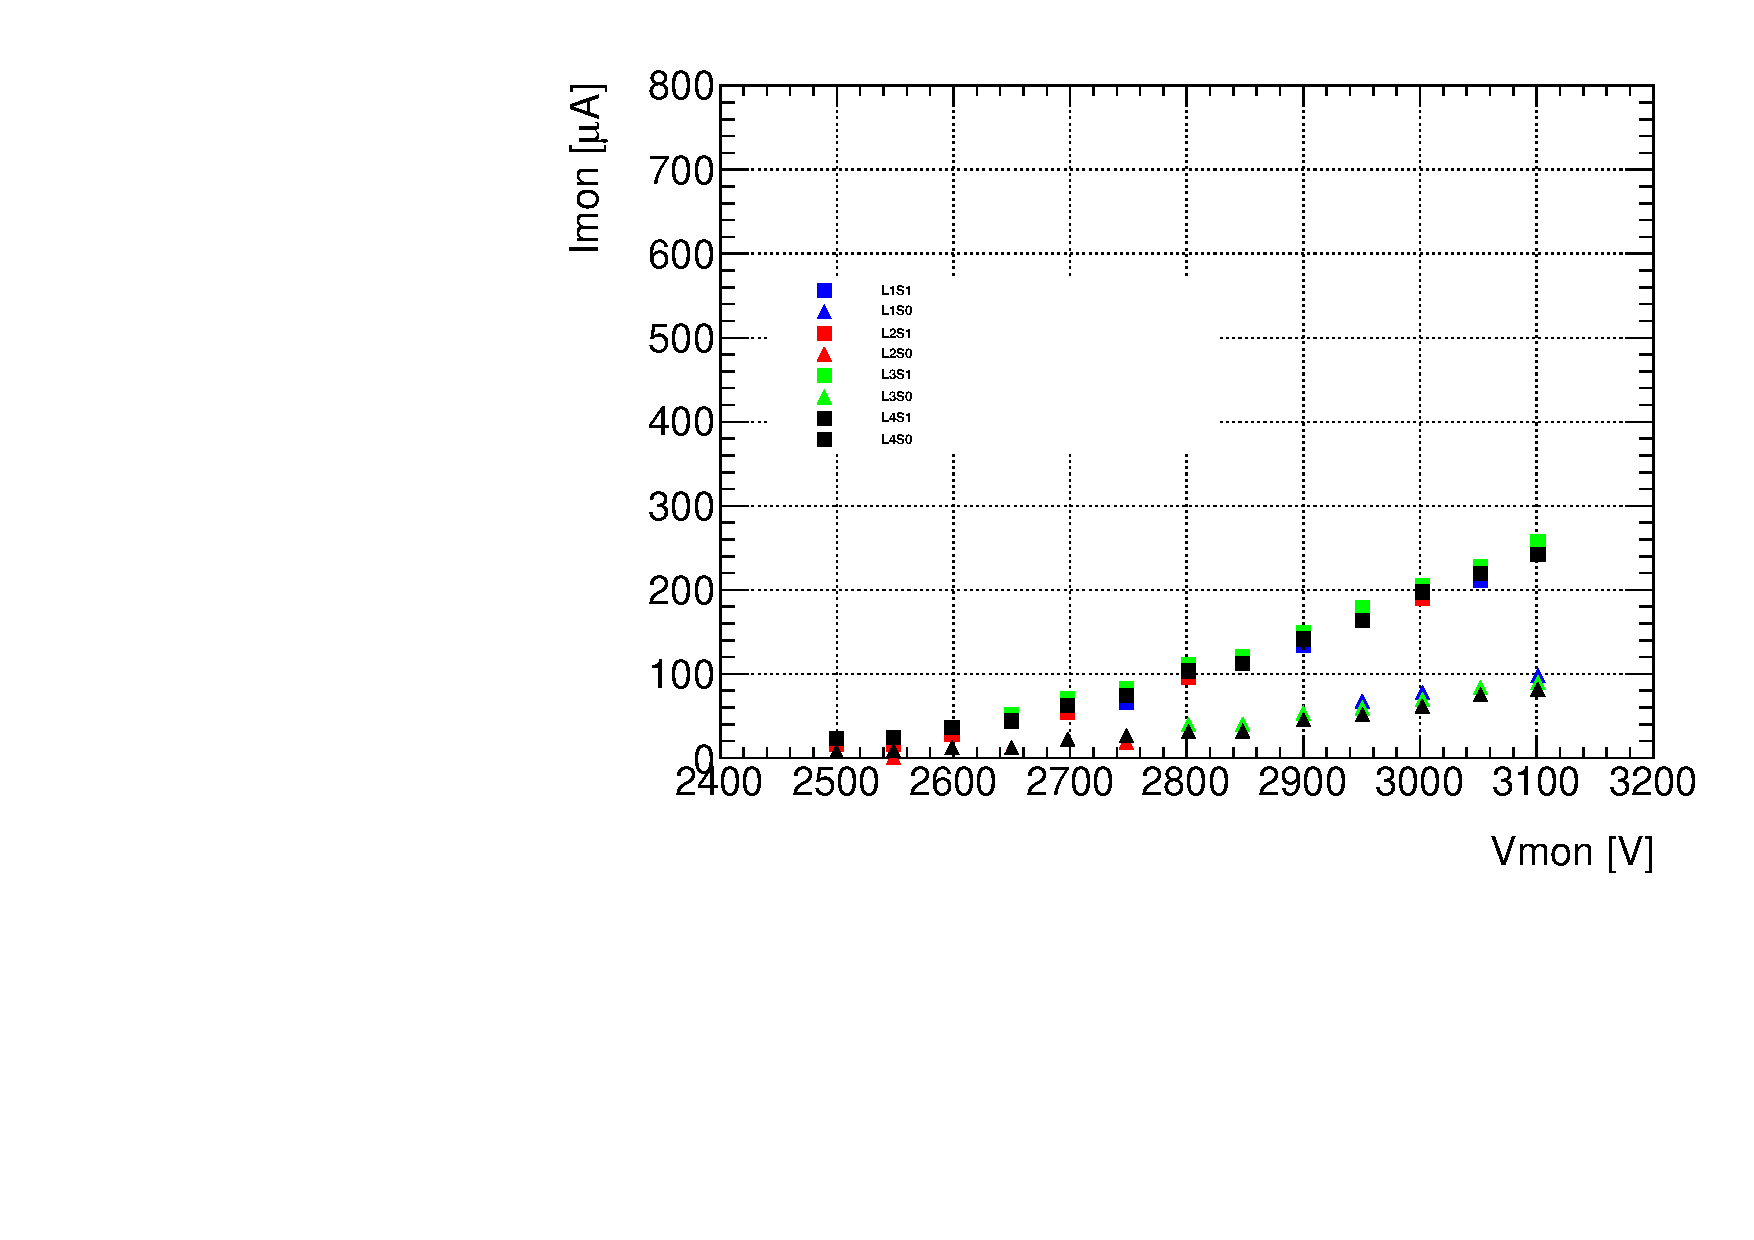
\includegraphics[width=\textwidth]{QS1_I_att10.pdf}
				\caption{Attenuation factor: 10}\label{fig:att10}
			\end{subfigure}
			\hspace*{\fill}
			\caption{}\label{gifresult}
	\end{figure}

	Once the Monitor is set, the quadruplet is connected to the high voltage power supply. Each layer is internally divided
	in two sections, a small sector (S0) and large sector (S1). Each one of theses sector is powered independently on each
	channel from the CAEN High Voltage power supply A1833P (\SI{4}{kV}/\SI{2}{mA}). The current from each layer (two
	sectors each one)	was recorded with a resolution of \SI{0.1}{\micro A}. Four different attenuation filters were applied, and the results are shown in Figure
	\ref{gifresult}. \par
\begin{equation}\label{eqn:delta}
\Delta\%=\left(1-\frac{I_1/I_0}{A_1/A_0}\right)*100
\end{equation}


	\begin{table}[ht]\footnotesize
		\centering
		\begin{tabular*}{0.7\textwidth}{rrcrcrcrc}
		 & \multicolumn{2}{c}{Layer 1} &\multicolumn{2}{c}{ Layer 2} &\multicolumn{2}{c}{ Layer 3
		}&\multicolumn{2}{c}{Layer 4}\\
		\hline
		$A_1$/$A_0$&\multicolumn{2}{c}{2.58}&\multicolumn{2}{c}{ 2.85}&\multicolumn{2}{c}{ 3.13}&\multicolumn{2}{c}{3.47}\\
		Filter & $I_1$/$I_0$ & $\Delta$\%& $I_1$/$I_0$ & $\Delta$\%& $I_1$/$I_0$ &$\Delta$\%& $I_1$/$I_0$ & $\Delta$\%\\ 	
		\hline
		10 	&2.49 &3.5  &3.02 &6 		&3.01 &3.8 	&3.08	&11.2 \\
		4.6 &2.34	&9.3 	&2.87 &0.7	&2.73 &12.7 &2.87	&17.3 \\
		2.2	&2.29 &11.2 &2.79 &2.1	&2.68 &14.4 &2.67	&23.1 \\
		1		&2.22 &14 	&3.02 &6 		&2.45 &21.7 &2.49	&28.2 \\
		\hline
		\end{tabular*}
		\caption{Comparison between sensitive area ratio ($A_1$/$A_0$) from large and small sector with the ratio of current
		($I_1$/$I_0$) at 2.9kV. A percentage difference column ($\Delta \%$ defined in equation \ref{eqn:delta}) is calculated to
		highlight the incremental disagreement as the gamma rate increase.}\label{aratio}
	\end{table}
These results shows an linear dependece of voltage, with lower resistance as the rate of particles is increased. It is
important to notice, each wire group is connected to a \SI{10}{\mega\ohm} resistor, however not all the wires have the
same length (the chamber has a trapezoidal shape), having lower voltage drop from the external groups where the wires are shorter (collecting less
charge).\par
The table \ref{aratio} compare the area ratio between the internal sections of each chamber with the current registered
for each set of measurements. The effect on droping voltage appears to be the explanation of the incremental
	disagreement from the area ratio as the rate increase. The larger percentual difference is for the Layer 4 where the
	larger section is bigger than the previous ones, hence, the current ratio is lower.\par


	%----------------- SPATIAL RESOLUTION ---------------


	\section{Spatial Resolution}
	In order to achieve the precision reconstruction of tracks (offline) with a spatial resolution of about
	\unit{100}{\micro m} per sTGC layer, and fast trigger on the region of interest (ROI) with Pads, two test beams were done.\\
	In the spring of 2014, the Weizmann Institute of Science in Israel built the first full-size sTGC quadruplet detector of
	dimensions \unit{1.2x1.0}{m$^2$}. This prototype consists of four sTGC strip and pad layers and is constructed using the full
	specification of one of the quadruplets to be used in the NSW upgrade (the middle quadruplet of the small sector).
	The first test beam experiment took place at Fermilab with one goal in mind, determine the position resolution of a
	full-size sTGC.\\par
	\begin{figure}[!ht]
		\centering
		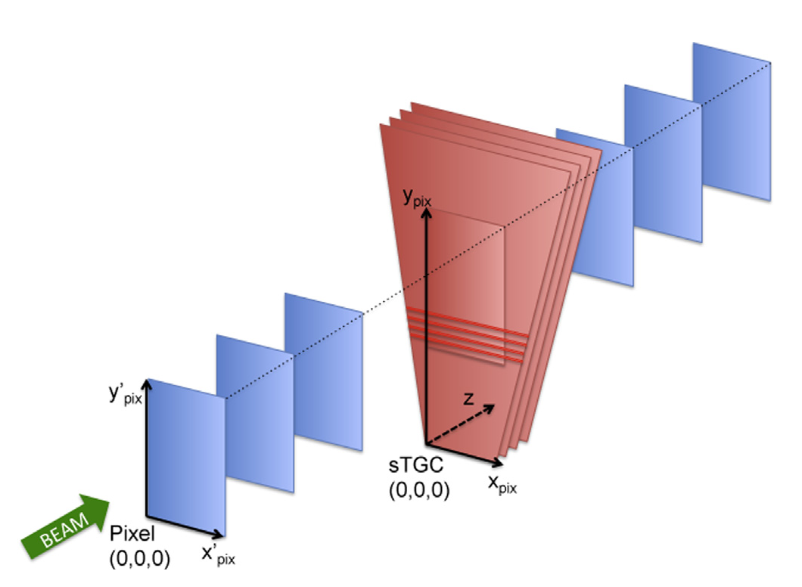
\includegraphics[width=0.5\textwidth]{telescope.png}
		\caption{\small Schematic diagram of the experimental setup at Fermilab and coordinate systems used. Three layers of silicon pixel sensors are positioned before and after the sTGC detector.The dimensions are not to scale.}\label{fig:telescope}
	\end{figure}
	EUDET pixel telescope were use as a reference for measure beam position, using the technology of 6 Minimum Ionizing MOS
	Active Pixel Sensor (Mimosa26) detectors with $\approx 5 \mu$m position resolution. Three in front of the beam, and three
	after the sTGC as is shown in fig.\ref{fig:telescope} with \unit{15}{cm} between them and \unit{64}{cm} between each arm.
	Each Mimosa26 detector has an active area of \unit{2.24}{cm$^2$} made of CMOS pixel
	matrix of 576 rows and 1152 columns with \unit{18.4}{\micro m} pitch.\par
	A \unit{32}{GeV} pion beam was used at rate of \unit{1}{kHz} over a spot of \unit{1}{cm$^2$} giving to the sTGC a very
	precise pion trajectory thanks to the EUDET telescope.
	Event triggering was controlled by a custom Trigger Logic Unit (TLU). The TLU received signals from two
	\unit{1x2}{cm$^2$}
	scintillators placed in front and behind the telescope. The TLU generated the trigger signal that was distributed to the
	telescope and the sTGC readout electronics, which consist of a first application-specific integrated circuit (ASIC)
	called VMM1 which has the ability to read out both positive (strips, pads) and negative (wires) polarity
	signals, on 64 individual readout channel. The VMM1 analog circuit features a charge amplifier stage followed by a
	shaper circuit and outputs the analog peak value (P) of the signal.The readout of the ASIC is zero suppressed and thus
	only peak values of channels with signals above a predefined threshold are read and at the same time the VMM1 may be
	programmed to provide the input signal amplitude of channels adjacent to a channel above threshold (neighbor-enable
	logic), which in case of the strips is strictly necessary due to the cluster size is about 3-5 strips.\par
	The precise position of a charged particle traversing an sTGC gas volume can be estimated from a Gaussian fit to the
	measured charge on adjacent readout strips (referred to as strip-clusters from here on). Given the strip pitch of
	\unit{3.2}{mm}
	and sTGC geometry, charges are typically induced on up to five adjacent strips. The spatial sampling of the total
	ionization signal over a small number of readout channels means that a precise knowledge of each individual readout
	channel baseline is necessary in order to achieve the best possible measured spatial resolution. The baseline of each
	individual readout channel was measured by making use of the neighbor-enabled logic of the VMM1 and its internal
	calibration system. Test pulses were sent on one readout channel with the neighbor-enabled logic on, and baseline
	values were obtained by reading out the analog peak values of the two channels adjacent to the one receiving a test
	pulse.\par
	The silicon pixel hit positions were then used for reconstructing straight three dimensional charged-particle tracks. A
	track quality parameter was obtained for each fitted pion track based on the $\chi^2$ of the track-fit. A small value of the track quality parameter corresponds to a straight track and a cut on this parameter can therefore be used to mitigate
	multiple scattering which are not considered in this analysis.
	\subsection{Analysis Model}
	\subsubsection{Pixel telescope analysis}
	In this model the intrinsic position resolution is obtained comparing the extrapolated beam trajectory from the pixel detectors
	with the measurements in each of the sTGC quad planes. Each layer is analyzed separately to reduce the effect of the
	multiple scattering and only tracks with $\chi^2<10$ are considered for the same reason. From fig.\ref{fig:telescope}
	you can see that the {\it y-axis} is defined perpendicular to the strips, therefore sTGC strip-clusters provide
	measurements of the particle position in the y-direction($y_{sTGC}$).
	The position resolution is directly related to the profile of induced charge on the strips. The particle position is
	estimated from a Gaussian fit to the induced charge distribution on the strips. The neighbor-enabled logic of the VMM1
	was used. Strip-clusters with induced charge in either 3, 4 or 5 adjacent strips are selected.\par
	The pixel telescope tracks provide both coordinates, x$_{pix}$ and $y_{pix}$ at the position of the sTGC layer studied. The
	spatial resolution measurement is obtained by fitting the residual distribution $y_{sTGC}$  and $y_{pix}$ with a Gaussian model.\par


	\begin{figure}[ht]
		\centering
		\hspace*{\fill}
		\begin{subfigure}[b]{0.45\textwidth}
			\centering
			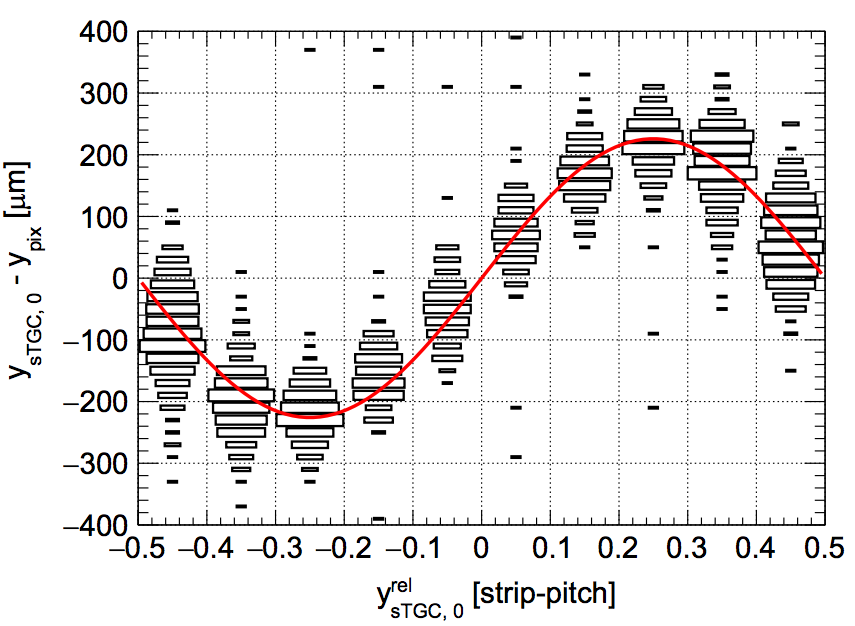
\includegraphics[width=\textwidth]{strip-pitch.png}
			\caption{The differential non-linearity for sTGC strip-clusters}\label{fig:pitchfit}
		\end{subfigure}
		\hfill
		\begin{subfigure}[b]{0.45\textwidth}
			\centering
			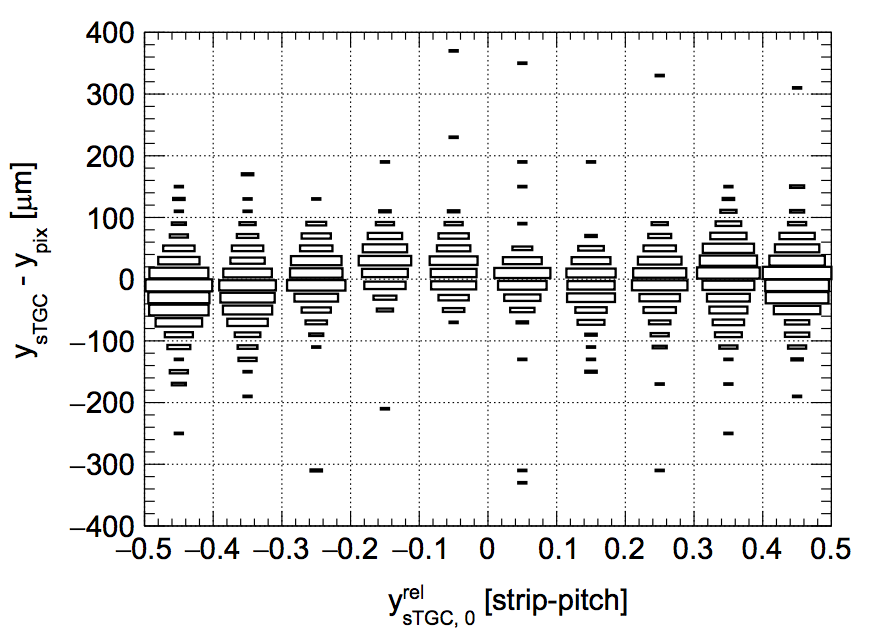
\includegraphics[width=\textwidth]{strip-aligned.png}
			\caption{The differential after sinusoidal correction is applied}\label{fig:pitchaligned}
		\end{subfigure}
		\hspace*{\fill}
		\caption{Charge distribution over strip-pitch}\label{fig:strip-pitch}
	\end{figure}


	The charge measured on the strips of the sTGC detector results from a spatial sampling and discretization of the induced
	charge. The process of reconstructing the sTGC strip-cluster position from this sampling introduces a differential
	non-linearity effect on the reconstructed strip-cluster position. The deviation of the measured strip-cluster position
	from the expected position (estimated by the pixel telescope track) depends on the strip-cluster position relative to
	the strips.
	This dependence is clearly seen in the two dimensional distributions in Fig.\ref{fig:pitchfit}. It shows the y-residual versus
	strip-cluster position relative to the closest inter-strip gap center $y_{sTGC,0}^{rel}$. This effect is corrected using
	a sinusoidal function.
	\begin{equation}
	 y_{sTGC} = y_{sTGC,0}-a_i\sin \left(2\pi y_{sTGC,0}^{rel}\right)
	\end{equation}
	where $y_{sTGC,0}$ is the strip-cluster mean resulting from the Gaussian fit and $y_{sTGC}$ is the corrected particle
	position estimator. The amplitude parameters are denoted $a_i$ for the 3,4 and 5 strip-multiplicity (cluster size). These
	amplitude parameters are free parameters in the fit. The values of the amplitude parameters obtained from the fit to
	data are compatible with being equal for the three strip-cluster multiplicity as shown in table \ref{table}.\par

	\begin{table}
		\centering
		\caption{Fit parameters per cluster size}\label{table}
		\begin{tabular}{cc}
		\hline
		Strip-cluster multiplicity $i$ & Amplitude parameter $a_i$\\
		\hline
		3 & 205 $\pm$ 9\\
		4 & 206 $\pm$ 4\\
		5 & 211 $\pm$ 5\\
		\hline
		\end{tabular}
	\end{table}

	The correction function is therefore universal and is shown in Fig.\ref{fig:pitchfit}. The two dimensional
	distribution after the correction is applied was to be reasonably flat as shown in Fig.\ref{fig:pitchaligned}.\par
	The alignment of the coordinate system of the pixel telescope with respect to the above-defined coordinate system of
	the sTGC layer also affects the measured residual distribution. A simple two-parameter model is used to account for
	translations and rotations of the two coordinate systems with respect to each other. Both the alignment correction and
	the differential non-linearity correction are included {\it in situ} in the analysis. The alignment correction is
	introduced in the model by expressing the pixel track position in the sTGC-layer coordinate system $y_{pix}$, is a
	function of the track position in the pixel telescope coordinate system $x_{pix}'$ and $y_{pix}'$, and two misalignment
	parameters $\delta y$ and $\phi_{xy}$, as follows:
	\begin{equation}
	y_{pix}=-x_{pix}' \sin \phi_{xy} + y_{pix}'\cos \phi_{xy}+\delta y
	\end{equation}
	The variable $\delta y$ corresponds to a misalignment along the y-axis of the sTGC coordinate system, and $\phi_{xy}$
	corresponds to a rotation of the telescope coordinate system in the x-y plane around the z-axis of the sTGC coordinate
	system. Translation and rotation misalignment along and around the other axis are not taken into account in this model,
	since they are expected to have a small impact on the determination of the intrinsic position resolution.\par


	\begin{figure}[ht]
		\centering
		\hspace*{\fill}
		\begin{subfigure}[b]{0.42\textwidth}
			\centering
			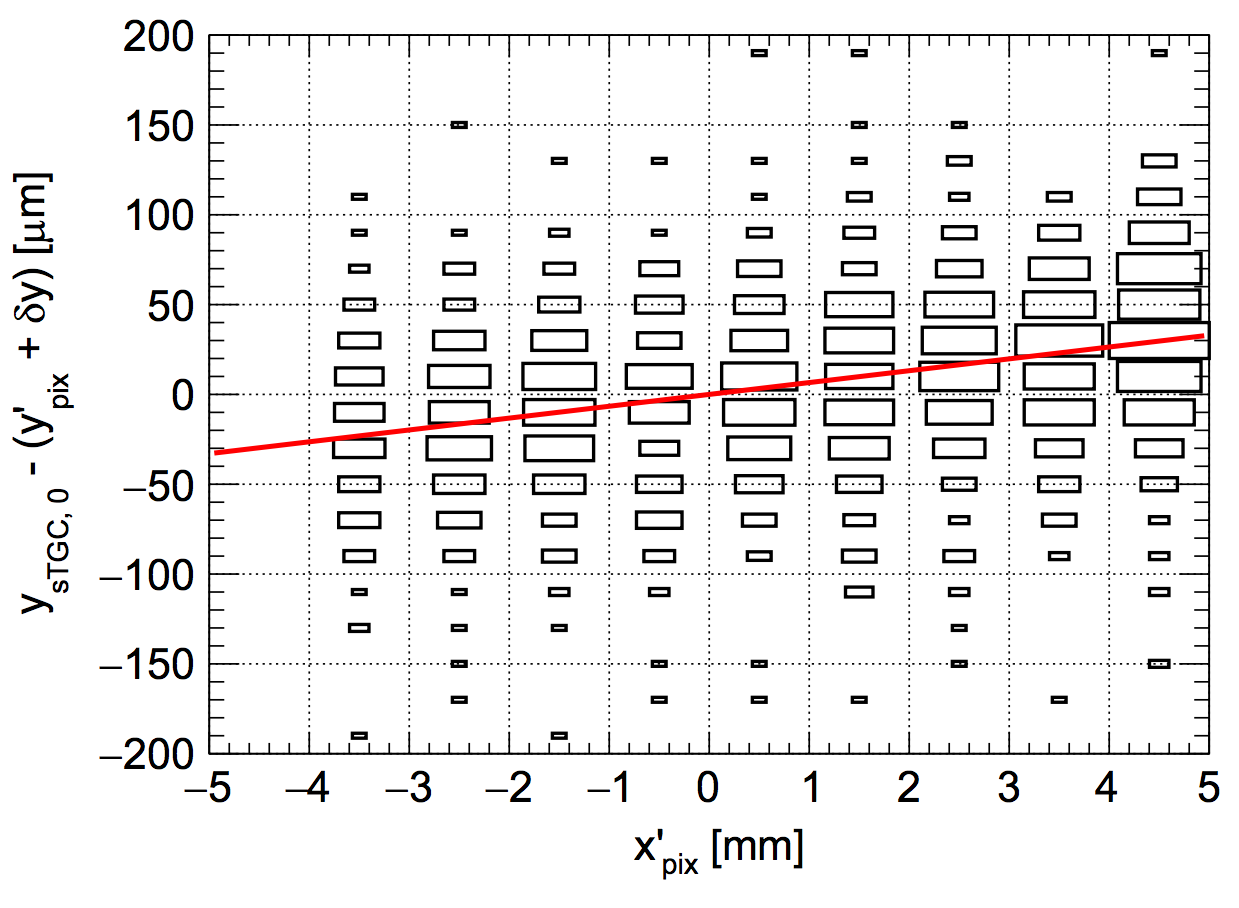
\includegraphics[width=\textwidth]{y-xplane.png}
			\caption{Residual y against x position on pixel telescope.}\label{xyplanefit}
		\end{subfigure}
		\hfill
		\begin{subfigure}[b]{0.42\textwidth}
			\centering
			\includegraphics[width=\textwidth]{y-xplanerotate.png}
			\caption{After rotation and translation applied}\label{xrotate}
		\end{subfigure}
		\hspace*{\fill}
		\caption{Coordinate system correction}\label{rotation}
	\end{figure}
	On the figure\ref{xyplanefit} is possible to observe the y-residual mean increase linearly as a function of the x
	position on the telescope called x$'_{pix}$, which is evidence for a small rotation between the two coordinate systems. 
	The red line represents the correction applied to this dataset. Accounting for this correction results in a distribution
	that is independent of x$'_{pix}$ on figure \ref{xrotate}.\par
	After all the corrections applied, the calculations for the intrinsic resolutions are taking each layer from the sTGC
	and comparing the residual distribution, and fitted by a double Gaussian function, where the first one represent the core
	of the residual distribution and the second is a wider Gaussian which represent some reconstructed strip-cluster from
	background sources.
	\begin{eqnarray*}
	F_i &=& F_i(y_{sTGC,0}, y_{sTGC,0}^{rel}, x'_{pix},y'_{pix};\delta y,\phi_{xy},a_i,\sigma,f,\sigma_w)\\
			&=& f G(y_{sTGC}-y_{pix};0,\sigma) + (1-f)G(y_{sTGC}-y_{pix};0,\sigma_w)
	\end{eqnarray*}
	\begin{figure}[ht]
	\centering
	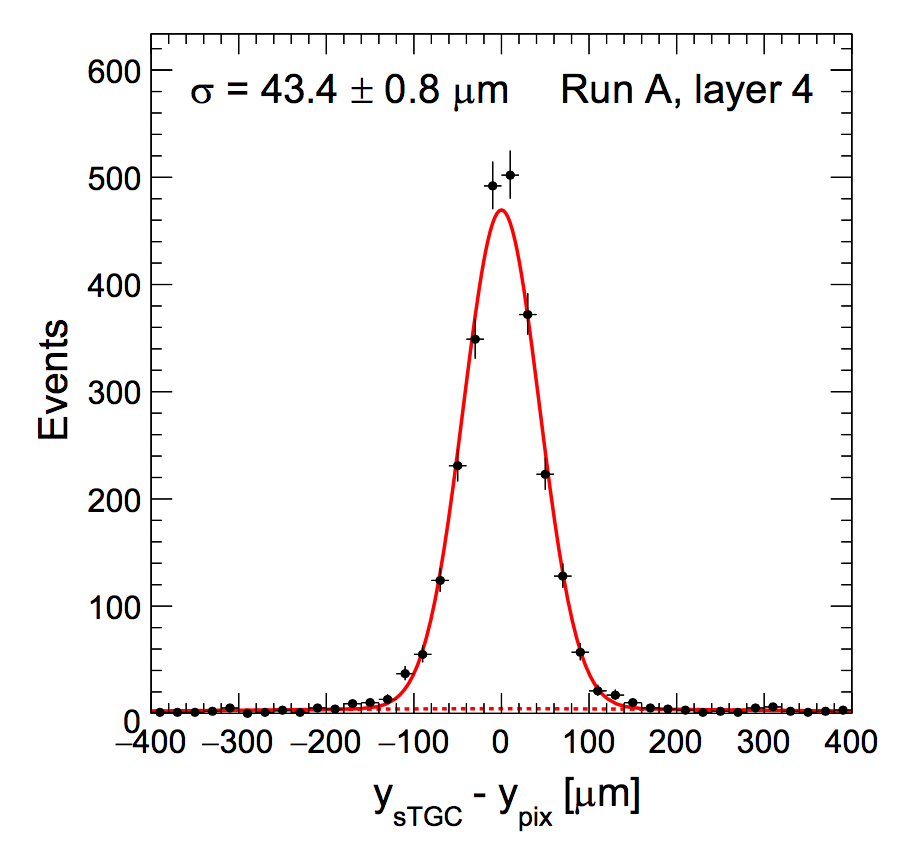
\includegraphics[width=0.4\textwidth]{resTelescope.png}
	\caption{Intrinsic resolution of layer 4, respect to pixel telescope.}\label{restelescope}
	\end{figure}

	\begin{figure}[ht]
	\centering
		\hspace*{\fill}
	\begin{subfigure}[b]{0.3\textwidth}
	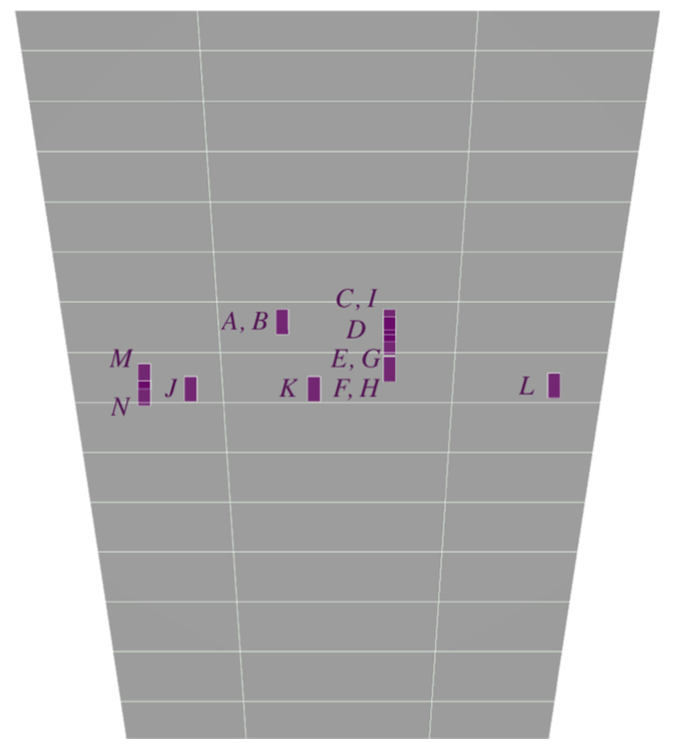
\includegraphics[width=\textwidth]{beampos.png}
	\caption{Beam position for different data sets on sTGC}\label{beampos}
	\end{subfigure}
	\hfill
	\begin{subfigure}[b]{0.6\textwidth}
	\centering
	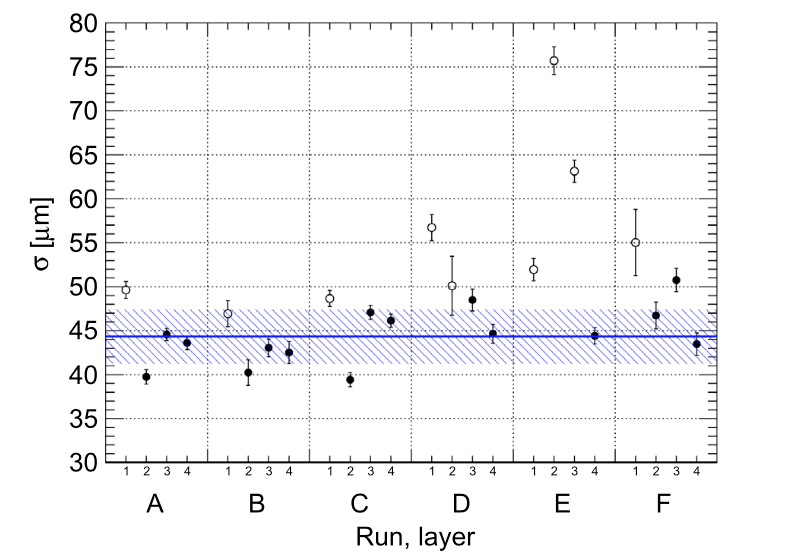
\includegraphics[width=\textwidth]{summaryTelescope.png}
	\caption{Summary of intrinsic resolution for each data set and layer of sTGC}\label{}
	\end{subfigure}
	\hspace*{\fill}
	\caption{Summary of pixel telescope analysis}\label{summary}
	\end{figure}


	On figure\ref{restelescope} a set of events shows the distribution presented before with a intrinsic resolution
	parameter $\sigma$ of about
	\unit{44}{\micro m} for a representative data taking run and sTGC strip-layer, where on red is the narrow Gaussian fit
	and on braking red line the wider Gaussian fit. The fraction of the data parameterized by the narrow Gaussian and it is
	typically around 95\% with a RMS of about 2\%. The rest of data taking runs and its beam position can be observe on
	figure \ref{summary}, where the black circles represent the valid data and the open circles the runs with expected
	degradation due detector structure support or mis-calibrations.\par




	%----------------- STANDALONE ANALYSIS 	---------------


	\subsubsection{sTGC standalone analysis}
	\begin{figure}[ht]
	\centering
	\hspace*{\fill}
	\begin{subfigure}[b]{0.45\textwidth}
	\centering
	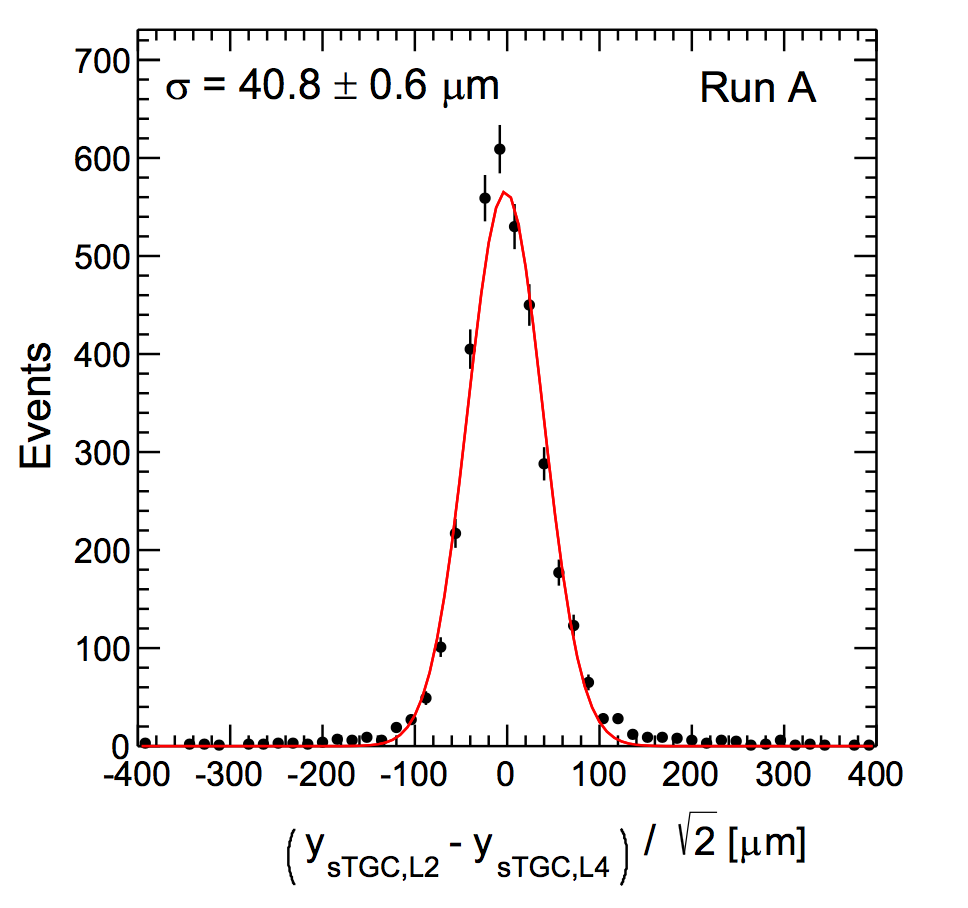
\includegraphics[width=\textwidth]{resStandalone.png}
	\caption{}\label{pairwise}
	\end{subfigure}
	\begin{subfigure}[b]{0.45\textwidth}
	\centering
	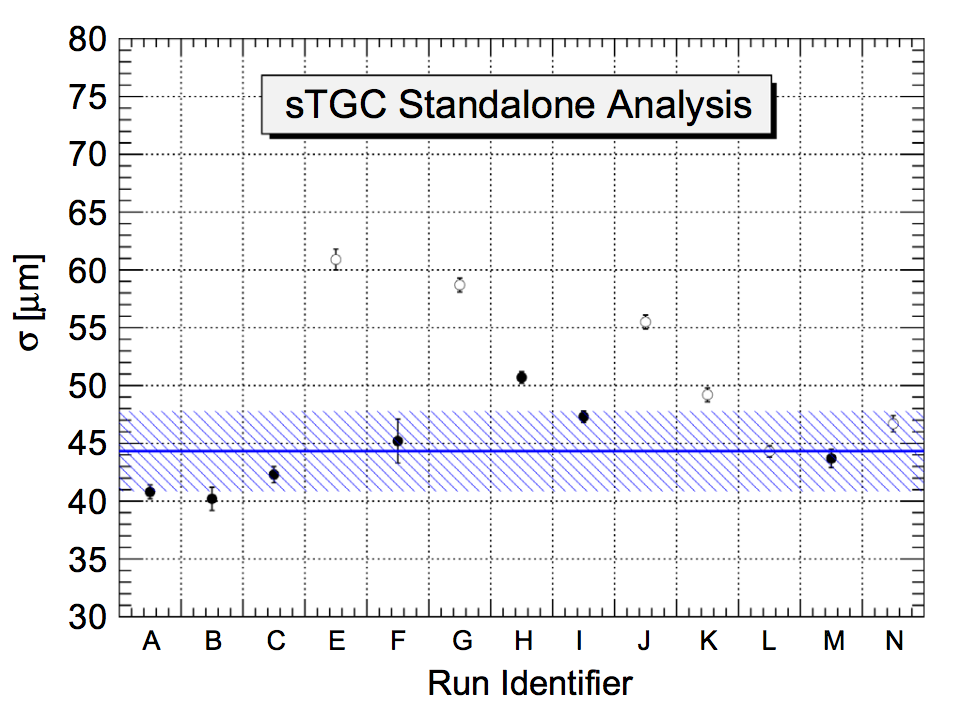
\includegraphics[width=\textwidth]{summaryStandalone.png}
	\caption{}\label{}
	\end{subfigure}
	\hspace*{\fill}
	\caption{}\label{}
	\end{figure}

	In this analysis the correction for the differential non-linearity respect to strip-pitch obtained before is kept,
	however the residual distribution of the y-position is calculated from two pairwise layer of the sTGC, therefore half of
	the variance of this distribution correspond to our parameter to estimate the intrinsic resolution for one layer, hence
	$\sigma = \sigma_{residual}/\sqrt{2}$ and a strip-layer position residual distribution for a representative sTGC
	standalone data taking run is shown in figure \ref{pairwise}. In this graph, a intrinsic resolution of $\sigma=40.8\pm0.8\mu m$ is obtained.\par 
	In summary for fourteen data sets, the intrinsic resolution with this analysis is about \unit{45}{\micro m}. The white open
circles on the graph \ref{summary} correspond to non-validate data due to wire-support position or mis-calibrations. The
hash band represent the RMS spread and the blue line the average.\par 



\section{Pad efficiency}
One of the new features of the small-strip Thin Gap Chamber compare to its previous version is the possibility to provide
a fast trigger for the Region of Interest from the \unit[8x50]{cm$^2$} pad area, where 3 out of 4 pads from a sTGC
quadruplet can confirm a particle candidate, therefore a track position can be obtained from the strips within this
area.\par
A test beam experiment was conducted at the CERN H6 beam line, using a \unit[130]{GeV} muon beam of about
\unit[4]{cm}
radius, a wider beam spot to test the characteristics of the pads. The setup is shown in figure \ref{padsetup} where the system was
triggered by a set of scintillators (in blue) with a \unit[12x12]{cm$^2$} coincidence area.\par
As explained before, for the beam tests a preliminary front-end electronics based on the VMM1 was used. This ASIC
provide a Time-over-threshold signal as digital output, however is also possible to get a analog pulses.
During the test beam, using the present configuration an inefficiency was observed related to small late charges from
the sTGC detector which may be not well adapted to the VMM1. An efficiency of 80-90\% was observe running at
\unit[100]{kHz/cm$^2$}.\par


\begin{figure}[ht]
\centering
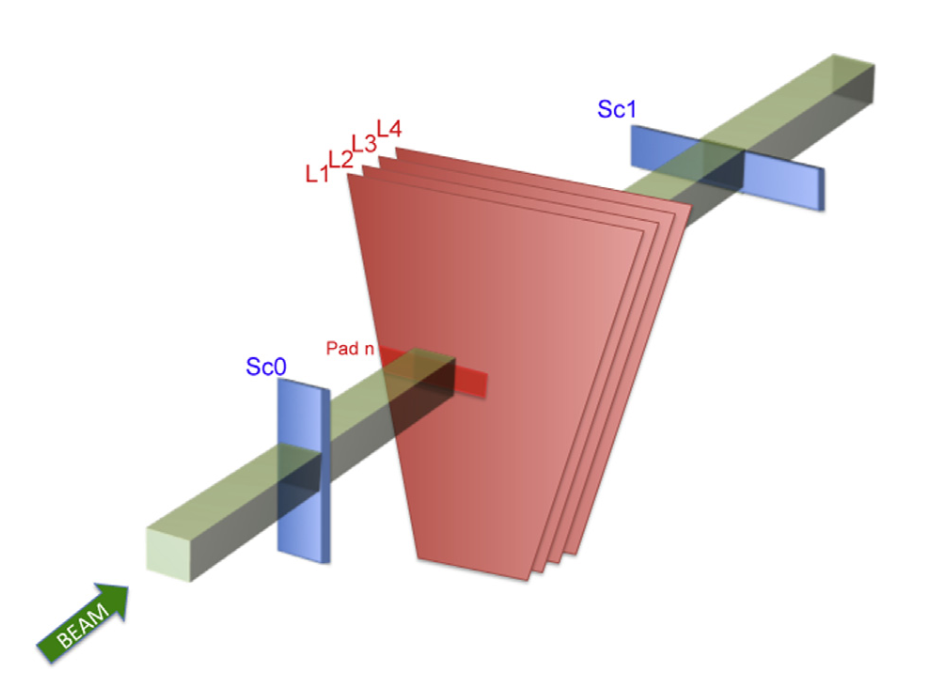
\includegraphics[width=0.6 \textwidth]{padSetup.png}
\caption{Setup for pad measurements, coincidence block on light green.}\label{padsetup}
\end{figure}


To ensure that no inefficiency was due the detector itself, the large cathode pads were used to estimate the detector
efficiency, which was measured by looking at the analog output of the front-end amplifier. The efficiency of the pad $n$
in the first layer was defined with respect to the coincidence of the trigger with a signal in the fully overlapping pad
of the second layer. \par



\begin{figure}[ht]
\centering
\hspace*{\fill}
\begin{subfigure}[b]{0.45\textwidth}
\centering
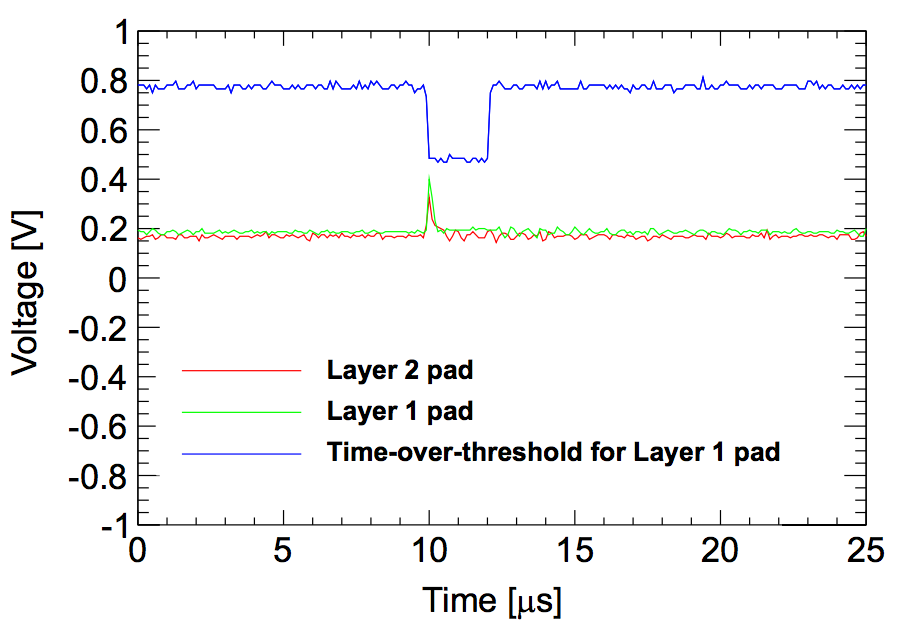
\includegraphics[width=\textwidth]{padnormal.png}
\caption{ToT signal from pad L1, pad L2 as a trigger}\label{scope1}
\end{subfigure}
\hfill
\begin{subfigure}[b]{0.45\textwidth}
\centering
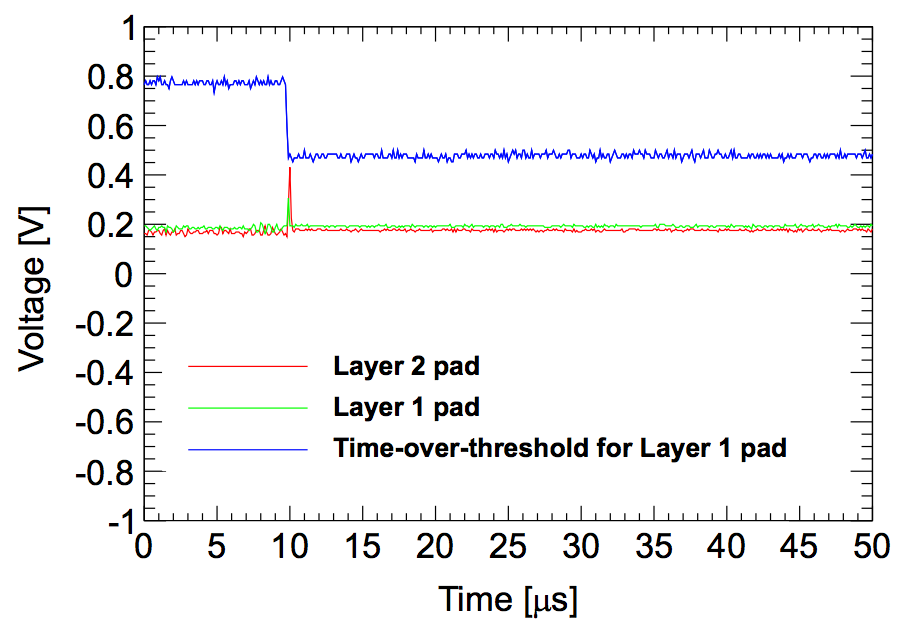
\includegraphics[width=\textwidth]{paddeadtime.png}
\caption{Large dead time on ToT signal from pad L1}\label{scope2}
\end{subfigure}
\hspace*{\fill}
\caption{Digital and analog signal from VMM1}\label{scope}
\end{figure}

Two examples from this configurations is shown on figure \ref{scope}, on the left a two analog signals from pads are
present with a ToT signal from layer 1 with about 2 \micro s length, meanwhile on the right picture a long ToT pulse with more
than 40 \micro s length when the two analog signal are present. By recording hundreds of triggered events using an
oscilloscope, the presence of a detector signal within the live-part of the front-end electronics (independent of the
signal threshold) was checked. This test confirmed that the detector was 100\% efficient.\par


\subsubsection{Charge sharing between pads}
\begin{figure}[ht]
\centering
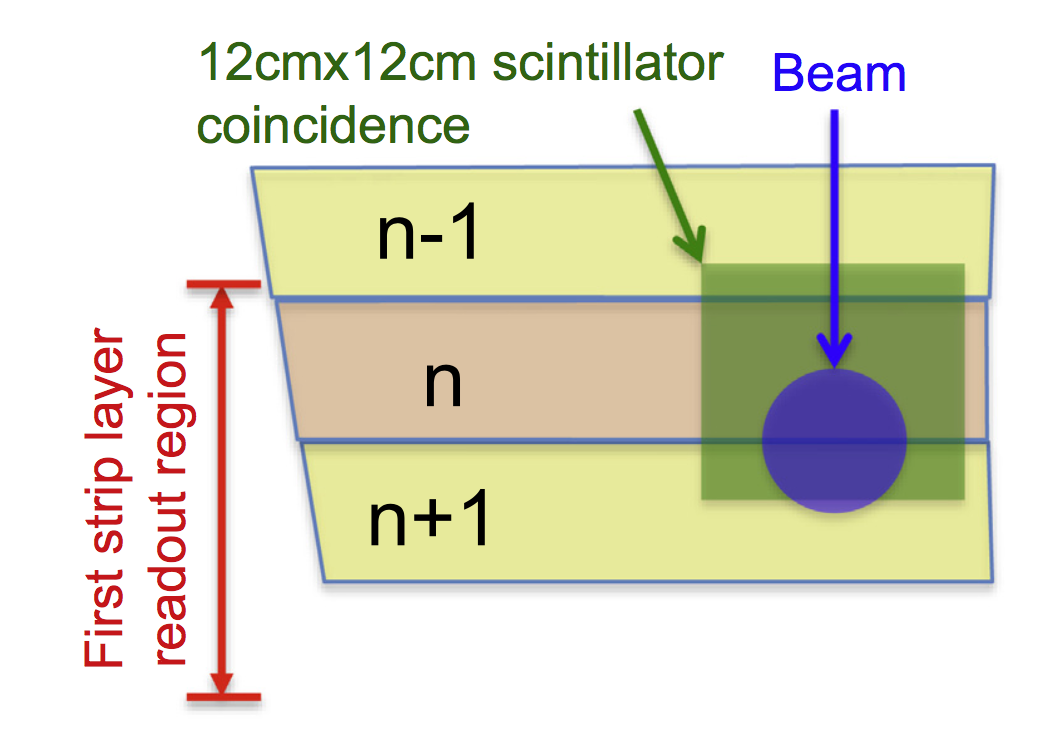
\includegraphics[width=.5\textwidth]{chargepos.png}
\caption{Pad region transition scheme}\label{chargepos}
\end{figure}

In manner to study the transition region between pads, the scintillator coincidence triggering area and the particle
beam were centered between pad $n$ and pad $n+1$ of the first layer, as illustrated in Figure \ref{chargepos}.\par
After applying timing quality requirements on the strip and pad hits, the channel baseline values are subtracted from
the analog peak values. Strip-clusters with induced charge in either 3,4 or 5 adjacent strips are selected and
calibrated in the same way as for the Fermilab beam test. Events with a single strip-cluster in the first layer and the
second layer are selected. The strip-cluster position (mean of the fitted Gaussian) in the first layer is used to define
the position of the particle going through the detector. The events are further required to contain a hit above
threshold on either pad $n$ or pad $n+1$. The charge fraction ($F$) is defined using the analog peak values ($P$) of the two
adjacent pads:
\begin{equation}
F = \frac{P_n - P_{n+1}}{P_n + P_{n+1}}
\end{equation}

\begin{figure}[ht]
\centering
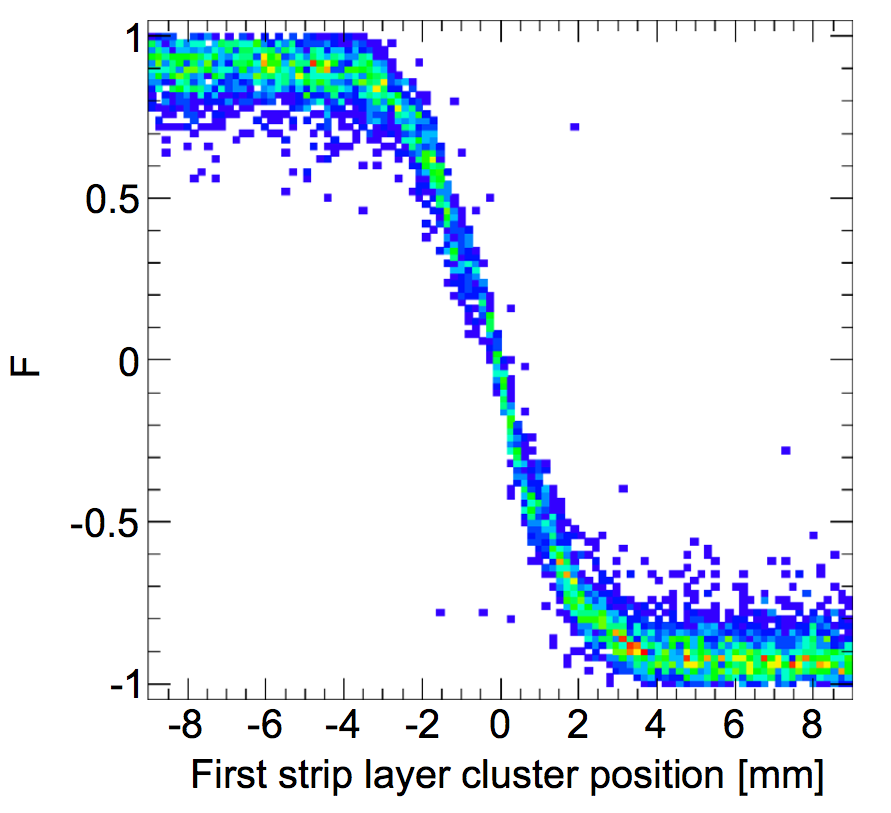
\includegraphics[width=0.5\textwidth]{chargeSharing.png}
\caption{Charge Sharing distribution}\label{chargeSharing}
\end{figure}

Figure \ref{chargeSharing} shows the charge fraction as a function of the position with respect to the center of the
transition region, where the two pads share more than 70\% of the induced charge, spans about \unit{4}{mm}.




\section{Summary}
The spatial resolutions and pad efficiency results has been published in ``Performance of a full-size small-strip thin gap chamber prototype
for the ATLAS new small wheel muon upgrade"
	\begin{itemize}
	\item A improvement of the dead time on the electronic readout must be done
	\item A cosmic muon test is remaining to provide the efficiency map for the module 0
	\item A test with muons with high background must be made with module 0, with the new readout electronics.
	\end{itemize}
